\documentclass{article}
\usepackage[a5paper, total={5in, 7.5in}]{geometry}
%\usepackage{input}
\usepackage{preamble}
%\usepackage{graphicx}

\begin{document}

\begin{titlepage}
    \centering
    \topskip0pt
    \vspace*{\fill}
    
    {\sl\large Классы при механико-математическом факультете МГУ} \medskip

    {\sl\large Школа 54}

    \vspace*{4cm}

    \begin{spacing}{1}
        \LARGE\bfseries Записи лекций Летней Школы\par по Программированию
    \end{spacing}
    \smallskip
    
    {\Large С.\,С.\,Князевский}
    \vspace{.6cm}
    
    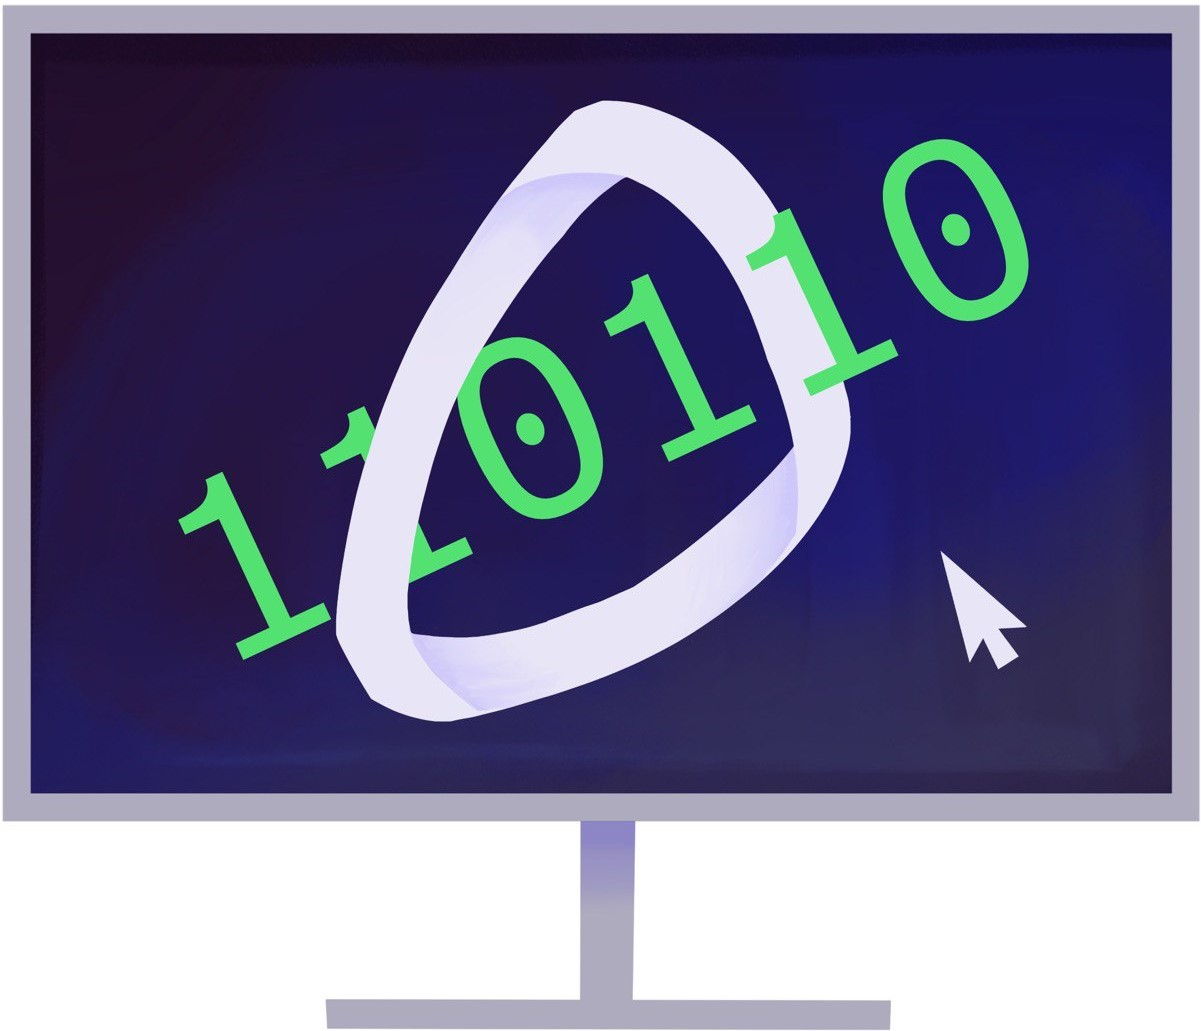
\includegraphics[width=0.4\textwidth]{./img/logo.jpg}

    \vspace*{4cm}

    {\large Красновидово}\medskip
    
    {\large 10 --- 24 августа, 2024 год}
    \vspace*{\fill}
\end{titlepage}

\thispagestyle{empty}

\begin{abstract}
    Данные материалы являются конспектом лекций, прочитанных в Летней школе по программированию в 2024\,г. Сергеем Сергеевичем Князевским и студентами механико-математического факультета МГУ им. М.\,В.\,Ломоносова: Пшеничным Никитой, Клочковым Иваном и Хакамовым Рамилем. Представленные в данной брошюре темы были выбраны с целью подготовки к олимпиадам по программированию различного уровня, начиная со школьного и заканчивая всероссийским.

    Набор осуществлял Пшеничный Никита при участии Льва Целомудрова. За редактуру и вычитку спасибо Сергею Сергеевичу Князевскому.
\end{abstract}

\newpage

\tableofcontents
\newpage

\section{Линейные алгоритмы}

\subsection{Префиксные суммы}

\begin{problem}
    Дан массив $\{a_0, a_1, \ldots, a_{n - 1}\}$. На $k$-ом из $m$ запросов даётся пара чисел $(l_k, r_k)$, т.\,ч. $0 \leqslant l_k \leqslant r_k < n$; нужно найти сумму $a_{l_k} + a_{l_k + 1} \hm + \ldots + a_{r_k}$.
\end{problem}

\begin{definition}
    \textit{Массивом префиксных сумм} массива $\{a_0, a_1, \ldots, a_{n - 1}\}$ называется массив (длины $n + 1$) $\{p_0, p_1, \ldots, p_n\}$, для которого $p_i \vcentcolon = \sum\limits_{j < i}a_j$. Иными словами, $p_0 = 0$, $p_1 = a_0$, $p_2 = a_0 + a_1$ и т.\,д.
\end{definition}

Нетрудно заметить, что $p_i = p_{i - 1} + a_{i - 1}$, поэтому массив префиксных сумм можно строить за линейное время. При этом, $\sum\limits_{i = l_k}^{r_k}a_i = p_{r_k + 1} - p_{l_k}$, т.\,е. ответ на каждый запрос даём за $O(1)$, поэтому итоговая сложность составляет $O(n + m)$.

\begin{minted}[linenos, mathescape]{cpp}
vector<int> p(n + 1); p[0] = 0;
for (int i = 1; i <= n; ++i)
    p[i] = p[i - 1] + a[i - 1]; // $p_0 = 0,\ p_i = a_0 + \ldots + a_{i - 1}$.
int m;
cin >> m;
while (m--)
{
    int l, r;
    cin >> l >> r;
    cout << p[r + 1] - p[l] << '\n';
}
\end{minted}

\subsection{Поиск оптимальной пары}

\begin{problem}
    В массиве $\{a_0, a_1, \ldots, a_{n - 1}\}$ найти пару $(i, j)$ такую, что $i < j$ и значение $a_j - a_i$ максимально возможное.
\end{problem}

\begin{wrapfigure}{r}{.35\textwidth}
    \begin{asy}
        defaultpen(fontsize(11pt));
        size(4cm);
        pair u = (1, -1), v = (3, 2), O = (0, 0);
        draw((O - 3 * u) -- (O) -- (O + v) -- (O + v + 2 * u));

        dot("$a_i$", O, 1.5 * dir(-60));
        dot("$a_j$", O + v, dir(45));
    \end{asy}
\end{wrapfigure}

Будем идти по массиву слева направо, \mbox{перебирая} правый элемент пары, а левый каждый раз выбирать наилучшим образом. Если правый элемент на данном шаге \mbox{имеет} индекс $j$, то наилучшим \mbox{левым} для него является $\min\{a_0, a_1, \ldots, a_{j - 1}\}$, ведь разность тем больше, чем меньше \mbox{вычитаемое}. При~этом, на~каждом новом шаге к рассмотрению добавляется ровно один элемент, поэтому для каждого правого элемента наилучший левый находим за~$O(1)$, поэтому всё решение работает за $O(n)$.

\begin{minted}[linenos, mathescape]{cpp}
int ibest = 0, jbest = 1;
int imin = 0;
for (int j = 2; j < n; ++j)
{
    if (a[j - 1] < a[imin]) imin = j - 1;
    if (a[j] - a[imin] > a[jbest] - a[ibest])
        ibest = imin, jbest = j;
}
cout << ibest << ' ' << jbest << '\n';
\end{minted}

\begin{problem}
    Даны массив $\{a_0, a_1, \ldots, a_{n - 1}\}$ и натуральное число $k$. Нужно найти пару $(i, j)$ такую, что $j - i \geqslant k$ и значение $a_i + a_j$ максимально возможное.
\end{problem}

Здесь применяем ту же идею, что и в задаче о поиске оптимальной \mbox{пары}, но с некоторыми модификациями. Во-первых, начинаем \mbox{перебирать} элемент $j$ не с начала, а с индекса $k$ (ведь до этого мы очевидно не~\mbox{найдём} подходящего индекса $i$). Во-вторых, лучшим элементом для $j$-го \mbox{теперь} является $\max\{a_0, a_1, \ldots, a_{j - k}\}$.

\subsection{Суммы на отрезках}

\begin{problem}
    В массиве $\{a_0, a_1, \ldots, a_{n - 1}\}$ нужно найти подотрезок $[a_l\ldots a_r]$, сумма на котором максимально возможная.
\end{problem}

Сразу отметим, что если данный массив состоит из неотрицательных чисел, то ответом всегда будет являться весь массив; сложности возникают, если разрешены отрицательные числа. Однако они разрешимы, \mbox{если} уметь решать первые две задачи в этой лекции. Для решения можно \mbox{предпосчитать} массив префиксных сумм данного массива, а затем для~него решить задачу о нахождении оптимальной пары.

Предположим теперь, что нам нужно найти лишь саму максимальную сумму, а не отрезок, на котором она достигается. У такой задачи есть очень изящное решение. Построим последовательность:
\[
    s_0 \vcentcolon = 0,\quad s_i \vcentcolon = \max\{s_{i - 1} + a_{i - 1}, 0\}\ (1 \leqslant i \leqslant n).
\]

Фактически, мы просто накапливаем префиксную сумму, но если она становится отрицательной, мы ставим её в $0$.

\begin{statement}
    Максимальная сумма на подотрезке данного массива равна $\max\{s_0, \ldots, s_n\}$.
\end{statement}

\begin{proof}
    Точки $i$, в которых $s_i = 0$, назовём \textit{критическими}. Заметим, что каждое $s_i$ равно сумме на подотрезке от ближайшей слева критической точки до $i$ (совпадение этих точек допускается в случае, если точка $i$ сама является критической). Отметим, что для каждого $i$ такая точка определена, т.\,к. $s_0 = 0$; обозначим её через $i^\ast$. Докажем, что максимальная сумма достигается на одном из таких отрезков. \mbox{Рассмотрим} произвольный отрезок $[a_l\ldots a_r]$. Сумма на отрезке $[a_{l^\ast}\ldots a_l]$ равна $s_l$ и, как следствие, неотрицательна. Поэтому сумма на отрезке $[a_{l^\ast}\ldots a_r]$ не~меньше, чем на $[a_l\ldots a_r]$, так что достаточно смотреть только на отрезки, начинающиеся в критических точках.
\end{proof}

На самом деле, к описанному алгоритму тоже можно <<прикрутить>> нахождение отрезка, на котором достигается максимум. Искомый отрезок есть $[a_{j^\ast}\ldots a_j]$, где $j$ --- индекс максимального члена последовательности $\{s_i\}$, а $j^\ast$ --- ближайшая к нему слева критическая точка.

\begin{problem}
    В массиве $\{a_0, a_1, \ldots, a_{n - 1}\}$ неотрицательных чисел найти подотрезок $[a_l\ldots a_r]$, сумма на котором равна заданному значению $k$.
\end{problem}

Будем искать отрезок следующим образом. Начнём с отрезка $[a_0]$, \mbox{состоящим} из одного элемента. На каждом шаге если сумма на \mbox{отрезке} меньше $k$, будем двигать правую границу отрезка на $1$ вправо (при этом сумма на отрезке не уменьшится), если меньше --- сдвинем левую \mbox{границу} на $1$ вправо (при этом сумма на отрезке не увеличится). Из \mbox{принципа} \mbox{дискретной} непрерывности, мы либо найдём искомый отрезок, либо правый конец отрезка начнёт указывать на индекс $n$.

\begin{minted}[linenos, mathescape]{cpp}
int i = 0, j, s = a[0];
for (j = 0; j < n; )
{
    if (s == k) break;
    if (s < k)
    {
        ++j;
        if (j < n) s += a[j];
    }
    else
    {
        s -= a[i];
        ++i;
    }
}

if (s == k)
    cout << i << ' ' << j << '\n';
else
    cout << "NO SOLUTION\n";
\end{minted}

\section{Структуры данных в линейных решениях}

\tikzset{
    queue element/.style={
        draw,very thin,rounded corners,
        fill=yellow!30,
        minimum width=1cm,minimum height=.5cm,
        font=\footnotesize
    }
}

\subsection{Стек и его применения в задачах}

\begin{definition}
    \textit{Стек} --- структура данных, представляющая из себя упорядоченный набор элементов, в которой добавление новых \mbox{элементов} и удаление существующих производится с одного конца, называемого \textit{\mbox{вершиной} стека}.
\end{definition}

\begin{center}
    \begin{tikzpicture}
        \fill[green!20] (5.1,.35) rectangle (-.6,-.35);
        \draw[green,thick] (-.6,.35) -- (5.1,.35) |- (-.6,-.35);
        \foreach \i/\name in {1/C,2/B,3/A}
            \node[queue element] (\name) at (1.5*\i,0) {\name};
        \draw[<-] ([yshift=.2cm]C.north) -- ++ (0,.5) node[above] {\texttt{st.top()}};
        \path (-3.6,0) node[right] {\texttt{st.push(D)}};
        \node[queue element] (D) at (-1.5,1) {D};
        \draw[->, thick] (D.south) to[out=-90,in=180] (-.7,0);
    \end{tikzpicture}\hspace*{2cm}
    \medskip
    
    \hspace*{1cm}
    \begin{tikzpicture}
        \fill[green!20] (5.1,.35) rectangle (-.6,-.35);
        \draw[green,thick] (-.6,.35) -- (5.1,.35) |- (-.6,-.35);
        \foreach \i/\name in {0/D,1/C,2/B,3/A}
            \node[queue element] (\name) at (1.5*\i,0) {\name};
        \draw[<-] ([yshift=.2cm]D.north) -- ++ (0,.5) node[above] {\texttt{st.top()}};
        \draw[->, thick] (-.7,0) to[out=180,in=90] ++ (-.5,-1);
        \path (5.3,0) node[right] {\texttt{st.pop()}};
    \end{tikzpicture}
\end{center}

\begin{problem}
    Для каждого элемента массива $\{a_1, a_2, \ldots, a_n\}$ найти ближайший справа элемент, меньший него.
\end{problem}

Если решать <<в лоб>>, то максимальное количество операций равно 
\[(n - 1) + (n - 2) + \ldots + 1 = \frac{n(n - 1)}{2} = O(n^2),\]
достигается при отсортированном по возрастанию массиве.

Для линейного решения предварительно добавим в массив граничные элементы $a_0 \vcentcolon = -\infty$, $a_{n + 1} \vcentcolon = -\infty$ и создадим стек, положив в него индекс $0$. Будем идти по массиву $\{a_1, a_2, \ldots, a_{n + 1}\}$ слева направо и \mbox{сравнивать} каждый элемент массива $a_i$ с элементом массива, доступным по \mbox{верхнему} индексу стека. Пока $a_i$ меньше верхнего элемента стека, будем удалять этот верхний элемент и записывать $i$ в качестве ответа для него. Затем добавим $i$ в стек.

Обоснуем корректность этого алгоритма. Сначала заметим, что стек никогда не остаётся пустым и каждый элемент хоть раз будет в него добавлен (в силу того, что $a_0 = -\infty$). Также, для каждого элемента будет записан ответ (в силу того, что $a_{n + 1} = -\infty$). Записанный ответ является правильным, т.\,к. для каждого числа записывается первое, меньшее него.

\begin{minted}[linenos, mathescape]{cpp}
vector<int> ans(n + 2);
stack<int> st; st.push(0);
for (int i = 1; i < n + 2; ++i)
{
    while (a[st.top()] > a[i])
        ans[st.top()] = i, st.pop();
    st.push(i);
}
\end{minted}

\begin{problem}[Гистограмма]
    Дан массив $\{h_1, h_2, \ldots, h_n\}$, представленный в~виде гистограммы. Требуется найти наибольшую площадь прямоугольника, вписанного в эту гистограмму.
\end{problem}

Заметим, что искомый прямоугольник имеет высоту, совпадающую с~высотой одного из столбцов. Действительно, если это не так, то можно увеличить его площадь, подняв до нижнего столбца в гистограмме. Будем перебирать столбцы и для каждой из них находить левую и правую границы с помощью предыдущей задачи. Для каждого столбца это можно сделать заранее и ответами заполнить \mbox{массивы} $\{l_1, l_2, \ldots, l_n\}$ и $\{r_1, r_2, \ldots, r_n\}$. Тогда площадь прямоугольника, покрывающего $i$-й столбец (высотой $h_i$) равна $S_i = h_i(r_i - l_i - 1)$.

\begin{problem}
    В массиве $\{\rlap{$\overbracket[.2mm]{\phantom{a_1, a_2, \ldots, a_k}}$}a_1, \underbracket[.2mm]{a_2, \ldots, a_k, a_{k + 1}}, \ldots, a_n\}$ найти минимум в скользящем окне шириной $k$.
\end{problem}

Решим задачу о нахождении ближайшего справа элемента меньше \mbox{текущего} и ответы запишем в массив $\{b_0, b_1, \ldots, b_{n + 1}\}$. Положим \mbox{$i = 1$} (указывает на первый элемент первого окна), а затем будем делать \mbox{замену} $i \mapsto b_i$, пока $b_i$ не выходит за границы окна. В конце $i$ будет указывать на~минимальный элемент в этом окне, т.\,к. $a_i$ меньше всех \mbox{элементов} \mbox{окна}, стоящих левее него, а первый элемент правее и \mbox{меньше} него уже не~\mbox{попадает} в окно. При переходе к новому окну если текущее значение $i$ в него не попадает, то ставим $i$ на позицию первого элемента нового окна.

Данный алгоритм работает за линейное время, т.\,к. $b_i > i$ для каждого индекса $i$. Таким образом, указатель на минимальный элемент окна не убывает. Всего элементов в массиве $n$, значит, изменений указателя не более $n$. Худший случай --- отсортированный по убыванию массив, на котором каждый раз мы двигаемся ровно на $1$ шаг.

\begin{minted}[linenos, mathescape]{cpp}
int i = 1;
vector<int> ans(n - k + 2);
for (int j = 1; j <= n - k + 1; ++j)
{
    if (i < j) i = j;
    while (b[i] < j + k) i = b[i];
    ans[j] = i;
}
\end{minted}

\begin{definition}
    Скобочная последовательность $s$ называется \textit{правильной}, если $s$ пуста или $s = (s^\prime)$, где $s^\prime$ --- правильная скобочная последовательность, или $s = s_1s_2$, где $s_1$ и $s_2$ --- правильные скобочные последовательности.
\end{definition}

\begin{problem}
    По данной скобочной последовательности проверить, является ли она правильной.
\end{problem}

% Заведём стек, в который изначально добавим первый символ данной последовательности. Далее будем идти по символам этой строки и если встретили закрывающую скобку, то сверху стека должна быть открывающая (соответствующая этой закрывающей). Тогда удалим этот элемент стека, а иначе добавим новый символ в стек. Если по окончании стек пуст, то наша скобочная последовательность правильная, иначе --- нет.

Заведём стек. Последовательно перебираем символы строки. Если встречаем открывающую скобку, добавляем её в стек, а если увидели закрывающую скобку, то сверху стека должна быть открывающая, парная текущей закрывающей. Тогда удалим эту открывающую скобку из стека. Если по окончании стек не пустой или во время работы не нашли парную для какой-то закрывающей скобки, данная скобочная последовательность не является правильной; иначе --- является.

\subsection{Очередь}

\begin{definition}
    \textit{Очередь} --- это структура данных, добавление и удаление элементов в которой происходит так, что первым из очереди удаляется элемент, который был помещен туда первым. У очереди имеется \textit{хвост}, куда добавляются элементы, и \textit{голова}, откуда они удаляются. 
\end{definition}

\begin{center}
    \begin{tikzpicture}
        \fill[green!20] (5.1,.35) rectangle (-.6,-.35);
        \draw[green,thick,>->] (-.6,.35) -- (5.1,.35);
        \draw[green,thick,>->] (-.6,-.35) -- (5.1,-.35);
        \foreach \i/\name in {1/C,2/B,3/A}
            \node[queue element] (\name) at (1.5*\i,0) {\name};
        \draw[<-] ([yshift=.2cm]A.north) -- ++ (0,.5) node[above] {\texttt{q.front()}};
        \path (-3.6,0) node[right] {\texttt{q.push(D)}};
        \node[queue element] (D) at (-1.5,1) {D};
        \draw[->, thick] (D.south) to[out=-90,in=180] (-.7,0);
    \end{tikzpicture}
    \hspace{2cm}

    \hspace{1cm}
    \begin{tikzpicture}
        \fill[green!20] (5.1,.35) rectangle (-.6,-.35);
        \draw[green,thick,>->] (-.6,.35) -- (5.1,.35);
        \draw[green,thick,>->] (-.6,-.35) -- (5.1,-.35);
        \foreach \i/\name in {0/D,1/C,2/B,3/A}
            \node[queue element] (\name) at (1.5*\i,0) {\name};
        \draw[<-] ([yshift=.2cm]A.north) -- ++ (0,.5) node[above] {\texttt{q.front()}};
        \draw[->, thick] (5.2,0) to[out=0,in=90] ++ (.5,-1);
        \path (5.5,0) node[right] {\texttt{q.pop()}};
    \end{tikzpicture}
\end{center}

Одним из основных применений очереди является реализация поиска в ширину, про это будет рассказано позже.

\subsection{Дек и второе решение задачи о минимуме в окне}

\begin{definition}
    \textit{Дек} --- структура данных, представляющая из себя \mbox{список} элементов, в которой добавление новых элементов и удаление \mbox{существующих} производится с обоих концов. 
\end{definition}

\begin{center}
    \begin{tikzpicture}[scale=.75, every node/.style={scale=.75}]
        \fill[green!20] (5.1,.35) rectangle (-.6,-.35);
        \draw[green,thick] (-.6,.35) -- (5.1,.35);
        \draw[green,thick] (-.6,-.35) -- (5.1,-.35);
        \foreach \i/\name in {0/D,1/C,2/B,3/A}
            \node[queue element] (\name) at (1.5*\i,0) {\name};
        \foreach \i in {0,1,2,3}
            \path (1.5*\i-.23,-.6) node [right] {\footnotesize $\i$};
        \draw[<-] ([yshift=.2cm]A.north) -- ++ (0,.5) node[above] {\texttt{deq.back()}};
        \draw[<-] ([yshift=.2cm]D.north) -- ++ (0,.5) node[above] {\texttt{deq.front()}};
        \path (-5.4,-1.2) node[right] {\texttt{deq.pop$\_$front()}};
        \path (-5.7,1.2) node[right] {\texttt{deq.push$\_$front(D)}};
        \draw[->, thick] (-.7,0) to[out=185,in=90] ++ (-3,-1);
        \draw[<-, thick] (-.7,0) to[out=175,in=-90] ++ (-3,1);
        \draw[->, thick] (5.2,0) to[out=-5,in=90] ++ (3,-1);
        \draw[<-, thick] (5.2,0) to[out=5,in=-90] ++ (3,1);
        \path (6.6,-1.2) node[right] {\texttt{deq.pop$\_$back()}};
        \path (6.4,1.2) node[right] {\texttt{deq.push$\_$back(A)}};
    \end{tikzpicture}
\end{center}

Отметим, что на дек бывает удобно смотреть как на двустороннюю очередь с индексацией.

Предложим другое решение задачи о поиске минимума в \mbox{скользящем} окне в массиве $\{a_0, a_1, \ldots, a_{n - 1}\}$ (в этот раз нам удобнее вести индексацию с $0$). Назовём элемент \textit{перспективным} для~данного окна, если в этом окне нет элементов правее и не больше него. Это условие необходимо для того, чтобы какой-то элемент был \mbox{минимумом} в~данном окне, поэтому этот минимум принадлежит множеству перспективных элементов. Заметим, что последовательность перспективных элементов неубывающая, а потому минимумом является первый элемент этой последовательности. Искать его будем так: заведём дек и сначала положим в него $0$ (\mbox{указывает} на первый элемент первого окна), а каждый следующий элемент будем добавлять, предварительно удалив из дека все элементы, большие этого следующего. Для перехода к новому окну удалим из дека первый элемент предыдущего окна, если он там есть (при~этом он всегда будет в начале дека), и добавим последний элемент нового указанным способом.

\begin{minted}[linenos, mathescape]{cpp}
deque<int> deq;
for (int i = 0; i < n; ++i)
{
    if (i >= k && deq.front() == i - k) deq.pop_front();
    while (deq.size() && a[deq.back()] >= a[i])
        deq.pop_back();
    deq.push_back(i);
    if (i >= k - 1)
        ans.push_back(deq.front());
}
\end{minted}

Для каждого из вышеперечисленных контейнеров определены методы \texttt{size()}, возвращающий количество его элементов, и \texttt{empty()}, проверяющий его на пустоту.

\section{Бинарный и тернарный поиски}

\subsection{Основная идея}

Предположим, есть массив $\{a_0, a_1, \ldots, a_{n - 1}\}$ и некоторое монотонное свойство $P$ в том смысле, что найдётся такой $i_0 \in [0; n)$, что $P(a_i) = P(a_j)$ для любых $i, j < i_0$ и для любых $i, j \geqslant i_0$, но $P(a_i) \ne P(a_j)$ для любых $i, j$, т.\,ч. $i < i_0 \leqslant j$.

Наша задача --- найти этот индекс $i_0$. Мы будем делать это следующим образом. Зафиксируем начало и конец полуинтервала поиска: $l \vcentcolon = 0$, $r \vcentcolon = n$. Если $P\br{a_{\lfloor(l + r) / 2\rfloor}} = P(a_l)$, то индекс перехода $i_0$ находится где-то на второй половине полуинтервала; иначе --- на первой. Обновляем значения $l$ и $r$ в соответствии с новым интервалом поиска. Алгоритм продолжает работу до тех пор, пока $l < r + 1$ (т.\,е. множество $[l; r)$ непусто).

Каждый раз интервал поиска уменьшается в два раза, так что совершаем $O(\log n)$ действий, а точнее --- либо $\lceil\log_2n\rceil$, либо $\lfloor\log_2n\rfloor$. Наивное решение (пройти по всем элементам массива) имеет асимптотику $O(n)$.

\subsection{Реализация}

\begin{problem}
    Найти в отсортированном массиве $\{a_0, a_1, \ldots, a_{n - 1}\}$ элемент, равный $x$, или определить, что его там нет.
\end{problem}

Положим $
P(a_i) =
\begin{cases}
    1,&\text{если $a_i \geqslant x$},\\
    0,&\text{иначе}
\end{cases}
$. Находим граничный элемент следующим образом:

\begin{minted}[linenos, mathescape]{cpp}
int l = 0, r = n;
while (l < r + 1)
{
    int m = (l + r) / 2;
    if (a[m] > x)
        r = m;
    else
        l = m;
}
\end{minted}

\subsection{Вещественный бинарный поиск}

Пусть теперь нам дана некоторая функция $f: \R \to \R$. Известно, что она непрерывна на отрезке $[a; b]$ и $f(a) \cdot f(b) < 0$. Теорема из математического анализа говорит, что у этой функции есть корень на данном отрезке. Искать его можно так же бинарным поиском, только теперь будем выполняться, пока $r - l > \varepsilon$, где $\varepsilon$ выбирается исходя из необходимой в задаче погрешности.

\begin{minted}[linenos, mathescape]{cpp}
long double l = a, r = b;
long double eps = 1e-6; // ... например
while (r - l > eps)
{
    long double m = (l + r) / 2;
    if (f(m) >= 0)
        r = m;
    else
        l = m;
}
\end{minted}

А можно делать фиксированное количество итераций, при этом чтобы получить $k$ правильных цифр, необходимо выполнить не менее $k \cdot \log_210$ операций.

\subsection{Бинарный поиск по ответу}

\begin{problem}
    На прямой расположены $n$ стойл (даны их координаты на прямой), в которые необходимо расставить $k$ коров так, чтобы минимальное расстояние между коровами было как можно больше. Гарантируется, что $1 < k < n$.
\end{problem}

Если решать задачу в лоб, то вообще неясно, что делать. Вместо этого решим более простую задачу: предположим, что мы знаем это расстояние $x$, ближе которого коров ставить нельзя. Тогда сможем ли мы расставить всех коров в соответствие с условием? Заметим, что это свойство монотонно --- для каких-то маленьких $x$ коров точно можно расставить, а начиная с каких-то больших --- уже нельзя, поэтому эту границу можно искать бинарным поиском.

\begin{minted}[linenos, mathescape]{cpp}
bool check(int x)
{
    int cows = 1;
    int last_cow = a[0];
    for (int c : a)
    {
        if (c - last_cow >= x)
        {
            ++cows;
            last_cow = c;
        }
    }
    return (cows >= k);
}

int bin_search()
{
    // Предполагаем, что координаты
    // в массиве $a$ уже отсортированы
    int l = 0, r = a.back() - a[0] + 1;
    while (r - l > 1)
    {
        if (check(m))
            l = m;
        else
            r = m;
    }
    return l;
}
\end{minted}

\begin{problem}
    Есть два принтера. Один печатает лист раз в $x$ минут, другой --- раз в $y$ минут. За сколько минут они напечатают $n$ листов?
\end{problem}

Конечно, эту задачу можно решить формулой за $O(1)$. Однако если такую формулу придумать не получается, сведём задачу к обратной. Подумаем, как по числу минут $t$ понять, сколько листов напечатается за это время? Очень легко:
\[
    \lfloor\frac{t}{x}\rfloor + \lfloor\frac{t}{y}\rfloor.
\]

Ясно, что за $0$ минут $n$ листов наспечатать нельзя, а за $x \cdot n$ минут один только первый принтер успеет напечатать $n$ листов. Поэтому $0$ и $x \cdot n$ --- это подходящие начальные границы для бинарного поиска.

\subsection{Тернарный поиск}

Пусть дана функция $f(x)$ имеем ровно один \textit{экстремум} --- локальный максимум или локальный минимум на отрезке $[a; b]$. Требуется найти точку этого экстремума.

Возьмём любые две точки $m_1$ и $m_2$ на этом отрезке: $l < m_1 < m_2 < r$. Посчитаем значения функции $f(m_1)$ и $f(m_2)$. Дальше у нас получается три варианта:

\begin{enumerate}[nolistsep]
    \item Если окажется, что $f(m_1) < f(m_2)$, то искомый максимум может находиться только в правой части, т.\,е. на отрезке $[m_1; r]$;
    \item Если, наоборот, $f(m_1) > f(m_2)$, то искомый максимум может находиться только в левой части, т.\,е. на отрезке $[l; m_2]$;
    \item А если $f(m_1) = f(m_2)$, то максимум находится на отрезке $[m_1; m_2]$, однако этот случай в целях упрощения кода можно отнести к любому из двух предыдущих.
\end{enumerate}

Выполнение алгоритма завершается, когда отрезок поиска станет достаточно маленьким. Осталось заметить, что мы не накладывали никаких ограничений на выбор точек $m_1$ и $m_2$. От этого способа будет зависеть скорость сходимости (и возникающая погрешность). Можно выбирать точки так, чтобы отрезок $[l; r]$ делился ими на $3$ равные части:
\[
    m_1 = l + \frac{r - l}{3},\quad m_2 = r - \frac{r - l}{3}.
\]

При этом каждый раз отрезок будет уменьшаться в $3 / 2$ раза. Однако, можно выбирать $m_1$ и $m_2$ очень близко друг к другу (и к середине отрезка), тогда каждый раз будем уменьшать отрезок почти в $2$ раза.

В случае целочисленного аргумента, отрезок $[l; r]$ становится дискретным, однако в силу отсутствия ограничений на выбор точек $m_1$ и $m_2$ корректность алгоритма не нарушается. Критерий остановки теперь --- $r - l < 3$, ведь в таком случае уже невозможно выбрать точки $m_1$ и $m_2$ удовлетворяли необходимому нам условию.


\section{STL}

\subsection{Множество}

\begin{center}
\tikzset{every loop/.style={min distance=15mm,looseness=10}}
\begin{tikzpicture}[-latex ,auto ,node distance =0.7cm and 5cm, on grid,semithick ,
state/.style ={circle, draw, color=blue!80 , fill=blue!80, text=white , minimum width =0.2 cm}, scale=.8, every node/.style={scale=.8}]
\path (0, 0) node[state] (a1) [label=left:$\alpha_1$]{};
\path (0, -.7) node[state] (a2) [label=left:$\alpha_2$]{};
\path (0, -1.4) node[state] (a3) [label=left:$\alpha_3$]{};
\path (.309, -1.9) node (adots) [label=left:$\vdots$]{};
\path (0, -1.4) node[state] (a3) [label=left:$\alpha_3$]{};
\path (0, -3.3) node[state] (an) [label=left:$\alpha_n$]{};
\path (0, -2.6) node[state, fill=blue!15, draw=blue!30] (ap) {};
\draw[<-, thick] (-.2,-2.6) to[out=180,in=0] ++ (-4.5, 0);
\path (-4.9, -2.6) node[state] (aprime) [label=left:$\alpha^\prime$]{};
\path (-2.9, -2.35) node {\texttt{se.insert($\alpha^\prime$)}};
\draw (0,-1.65) ellipse (1.4 and 2.8);
\draw[<-, thick] (.2,0) to[out=0,in=180] ++ (2, 0);
\draw[<-, thick] (.2,-3.3) to[out=0,in=180] ++ (2, 0);
\path (2.2, 0) node[right] (beg) {\texttt{se.begin()}};
\path (2.2, -3.28) node[right] (end) {\texttt{se.end()}};
\end{tikzpicture}
\end{center}

Множетсво инициализируется как \texttt{set<T> se}. Представляет собой стандартное математическое множетсво. Можно добавлять элементы с~помощью \texttt{se.insert($x$)}, удалять с помощью \texttt{se.erase($x$)} или \texttt{se.erase($p_x$)}, где $p_x$ --- указатель на элемент со значением $x$. Методы \texttt{se.begin()} и \texttt{se.end()} возвращают указатели на начальный и конечный элемент множества соответственно. Начальный элемент в множестве \texttt{int}-ов является минимальным в множестве. Метод \texttt{se.find($x$)} возвращает указатель на~элемент со значением $x$, то есть $p_x$. Если же такого элемента в множестве нет, то вернётся указатель на последний элемент --- \texttt{se.end()}. В STL есть такая структура данных, как мультимножество, \texttt{multiset<T>~mse}. Оно отличается от обычного множества тем, что может хранить неуникальные элементы. Теперь удаление элемента по значению влечёт удаление всех его вхождений.

Все операции работают за $O(\alpha \cdot \log n)$, где $n$ --- размер множества, а $\alpha$ --- оценка сравнения ключей. Например, для целых чисел $\alpha = O(1)$, а для строк $\alpha = O(\abs{s})$.

\subsection{Карта/словарь}

Карта представляет собой набор пар $(\alpha_i, \beta_i)$, в которых по умолчанию $\beta_i = 0$. Карта инициализируется как \texttt{map<T1, T2> ma}. При этом, к элементам можно обращаться следующим образом: \texttt{ma[$\alpha_i$]$\, = \beta_i$}. Пары внутри \texttt{map}-а (как и элементы внутри \texttt{set}-а) сортируются по возрастанию. А пары сортируются по первому элементу, поэтому \texttt{ma.begin()} указывает на пару с наименьшим первым элементом.

\begin{center}
\tikzset{every loop/.style={min distance=15mm,looseness=10}}
\begin{tikzpicture}[-latex ,auto ,node distance =0.7cm and 5cm, on grid,semithick ,
state/.style ={circle, draw, color=blue!80, fill=blue!80, text=white , minimum width =0.2 cm},
state2/.style ={circle, draw, color=red!80 , fill=red!80, text=white , minimum width =0.2 cm}]
\path (0, 0) node[state] (a1) [label=left:$\alpha_1$]{};
\path (0, -.7) node[state] (a2) [label=left:$\alpha_2$]{};
\path (0, -1.4) node[state] (a3) [label=left:$\alpha_3$]{};
\path (.309, -1.9) node (adots) [label=left:$\vdots$]{};
\path (0, -1.4) node[state] (a3) [label=left:$\alpha_3$]{};
\path (0, -2.6) node[state, fill=blue!15, draw=blue!30] (ap) [label=left:$\alpha_i$]{};
\path (.309, -3.1) node[] (adots2) [label=left:$\vdots$]{};
\path (0, -3.8) node[state] (an) [label=left:$\alpha_n$]{};
\draw[->, thick] (.2, 0) to[out = 0, in = 180] ++ (1.8, 0);
\draw[->, thick] (.2, -.7) to[out = 0, in = 180] ++ (1.8, 0);
\draw[->, thick] (.2, -1.4) to[out = 0, in = 180] ++ (1.8, 0);
\draw[->, thick] (.2, -2.6) to[out = 0, in = 180] ++ (1.8, 0);
\draw[->, thick] (.2, -3.8) to[out = 0, in = 180] ++ (1.8, 0);

\path (2.2, 0) node[state2] (a1) [label=right:$\beta_1$]{};
\path (2.2, -.7) node[state2] (a2) [label=right:$\beta_2$]{};
\path (2.2, -1.4) node[state2] (a3) [label=right:$\beta_3$]{};
\path (2.51, -1.9) node (adots) [label=left:$\vdots$]{};
\path (2.2, -1.4) node[state2] (a3) [label=right:$\beta_3$]{};
\path (2.2, -2.6) node[state2, fill=red!15, draw=red!30] (ap) [label=right:$\beta_i$]{};
\path (2.51, -3.1) node (adots2) [label=left:$\vdots$]{};
\path (2.2, -3.8) node[state2] (an) [label=right:$\beta_n$]{};
\end{tikzpicture}
\end{center}

Все операции в \texttt{map}-е работают за $O(\log n)$, даже получение элемента. Поэтому стоит минимизировать их количество. Контейнер \texttt{map} в полную силу раскрывается, если в качестве ключей использовать строки. Тогда мы строкам можем очень быстро сопоставлять числа. Хранить в массиве это было бы невозможно, так как строки могут состоять из очень большого количества символов; в \texttt{map}-е же такой проблемы не возникает.

\subsection{Очередь с приоритетом}

STL предоставляет также контейнер \texttt{priority\_queue}, который, помимо функционала обычной очереди, поддерживает определённый порядок элементов: в голове очереди (по \mintinline{cpp}{q.front()}) находится наибольший элемент. Инициализируется так: \texttt{priority\_queue<T> q}, поддерживает методы \texttt{front()} за $O(1)$ и \texttt{push\_back()}, \texttt{pop\_back()} за $O(\log n)$.


\section{Битовый бой}

\subsection{Двоичная система счисления}

\begin{definition}[Системы счисления]
    \[
        \overline{a_{n - 1}\ldots a_1 a_0}_x \vcentcolon = \sum\limits_{i = 0}^{n - 1} a_i\cdot x^i
    \]
\end{definition}

В компьютере числа хранятся в двоичной системе счисления, причём хранение отрицательных чисел производится с помощью, так называемого, \textit{обратного кода}. Первый бит отвечает за знак числа (для неотрицательных он равен $0$, для отрицательных $1$). Пусть имеем двоичное число  $A = 1101\underbrace{0\ldots0}_{28\, \text{нулей}}$. Как найти обратное к нему? Чтобы арифметика работала, нужно, чтобы такое число $B$ при сложении с $A$ давало $0$. Этого можно добиться переполнением, то есть, нам нужно получить число $1\underbrace{0\ldots0}_{32\, \text{нуля}}$, что~в типе \texttt{int} является нулём (ведь он хранит только 32 младших бита). Так, нам подойдёт число $B = 0011\underbrace{0\ldots0}_{28\,\text{нулей}}$.

\subsection{Битовые операции}

\begin{definition}
    \begin{enumerate}[nolistsep]
        \item \textit{Конъюнкция} --- побитовое <<и>> ($x\;\&\;y$);
        \item \textit{Дизъюнкция} --- побитовое <<или>> ($x\;\vert\;y$);
        \item \textit{XOR} --- сложение $\bmod\;2$ ($x \wedge y$);
        \item \textit{Инверсия} --- побитовое отрицание ($\sim x$);
        \item \textit{Побитовый сдвиг вправо} --- умножение на $2^k$ ($x\;\texttt{<<}\;k$);
        \item \textit{Побитовый сдвиг влево} --- целочисленное деление на $2^k$ ($x\;\texttt{>>}\;k$).
    \end{enumerate}
\end{definition}

\noindent
\begin{minipage}{.25\textwidth}
$$\def\arraystretch{.8}
\begin{array}{r}
\&
\begin{array}{r}
110100\\

100111\\
\end{array}\\
\hline
\def\arraystretch{.2}
\begin{array}{r}\\
100100
\end{array}
\end{array}
$$
\end{minipage}
\begin{minipage}{.25\textwidth}
$$\def\arraystretch{.8}
\begin{array}{r}
|
\begin{array}{r}
110100\\

100111\\
\end{array}\\
\hline
\def\arraystretch{.2}
\begin{array}{r}\\
110111
\end{array}
\end{array}
$$
\end{minipage}
\begin{minipage}{.25\textwidth}
$$\def\arraystretch{.8}
\begin{array}{r}
\wedge
\begin{array}{r}
110100\\

100111\\
\end{array}\\
\hline
\def\arraystretch{.2}
\begin{array}{r}\\
010011
\end{array}
\end{array}
$$
\end{minipage}
\begin{minipage}{.25\textwidth}
$$\def\arraystretch{.8}
\begin{array}{r}
\begin{array}{r}
{}\\
\sim110100
\end{array}\\
\hline
\def\arraystretch{.2}
\begin{array}{r}\\
001011
\end{array}
\end{array}
$$
\end{minipage}

\problem{Определить значение $i$-го бита числа $x$}

\solution{$x\;\&\;(1\;\texttt{<<}\;i)$}

\problem{Инвертировать $i$-й бит числа $x$}

\solution{$x \wedge (1\;\texttt{<<}\;i)$}

\subsection{Битовые маски}

Заметим, что любое множество (из не более чем 32 элементов) можно задавать двоичной строкой (элементы кодируются $1$ на соответствующих местах). Например, строка $0011001$ задаёт множество $\{0, 3, 4\}$. Заметим, что это даёт нам возможность быстро использовать операции над множествами (им соответствую операции над двоичными числами). Пусть $f$~---~функция, которая по битовой маске строит соответствующее ей множество, $A$ и $B$ --- некоторые множества. Некоторые примеры операций:

$$
    \begin{array}{l}
    A \cap B \leftarrow f^{-1}(A)\; \&\; f^{-1}(B),\\
    A \cup B \leftarrow f^{-1}(A)\; |\; f^{-1}(B),\\
    A\:\Delta\:B \leftarrow f^{-1}(A)\; \wedge\; f^{-1}(B),\\
    \overline{A} \leftarrow\ \sim f^{-1}(A),\\
    A \setminus B \leftarrow f^{-1}(A)\; \&\; (\sim f^{-1}(B)).
\end{array}$$

\subsection{Bitset-ы}

Т.\,к. часто приходится работать с большими множествами (количество элементов в которых больше 32 и даже 64), нам не подходят для хранения обычные числовые типы вроде \texttt{int} и \texttt{long long}. Как раз для этого существует \texttt{bitset<SIZE>} (\texttt{SIZE} --- обязательно константа). Он предоставляет все операции над двоичными числами (единственное условие --- они должны быть одинакового размера).

Помимо увеличенного размера двоичных чисел, \texttt{bitset}-ы нужны, чтобы уменьшать время работы операций, так как в нём биты хранятся не отдельно, а в составе байта (группами по 8 штук), поэтому операции с~\texttt{bitset}-ом работают с очень маленькой константой (как раз в 8 раз меньше, чем при применении битовых операций к обычным числам).


\section{Введение в графы. Обход в ширину}

Будем рассматривать граф $G$ с множеством вершин $V \vcentcolon = \{0, 1, \ldots, n \hm - 1\}$ и множеством рёбер $E$. 

\subsection{Способы хранения графов}

Есть несколько способов хранения графов, каждый из которых удобен в разных ситуациях.

\begin{enumerate}
    \item \textbf{Список рёбер}. Название говорит само за себя: заводится массив, в котором хранятся рёбра в виде пар инцидентных вершин. Применяется, например, в алгоритме Краскала (см.\,лекцию по СНМ).
    \item \textbf{Матрица смежности}. Заведём двумерный массив $a$ размера $n \times n$, заполненный следующим образом:
    \[
    a_{ij} =
    \begin{cases}
        1,&\text{если $(i, j) \in E$},\\
        0,&\text{иначе}.
    \end{cases}
    \]
    Отметим, что для неориентированного графа матрица смежности является симметрической.
    \item \textbf{Список смежности}. Заведём двумерный массив $a$ размера $n$, в котором по индексу $i$ хранится массив вершин, инцидентных $i$. Этот способ обычно удобнее всего, т.\,к. 1) удобнее всего получать соседей для каждой вершины; 2) суммарный размер $O(m)$, а не $O(n^2)$, что полезно, когда $m \sim n$.
\end{enumerate}

\subsection{Идея поиска в ширину}

При обходе в ширину мы идём по вершинам в порядке, в котором они бы сгорали, если поджечь начальную (каждую секунду огонь распространяется на соседние вершины). Моделируем данный процесс, пока не сгорит весь граф. Важно помнить, что мы не поджигаем уже горящие вершины. Т.\,к. огонь распространяется равномерно по кратчайшим путям, секунда, на которой сгорела $i$-я вершина --- это расстояние до неё.

\subsection{Реализация}

\begin{minted}[linenos, mathescape]{cpp}
// Список смежности графа $G$ размера $n$
vector<vector<int>> adj;
// Векторы для хранения расстояний до каждой вершины
// и её предков
vector<int> dist, parent;

void bfs(int start)
{
    queue<int> q; // Очередь для хранения горящих вершин
    dist.assign(n, INF);
    parent.assign(n, -1);
    q.push(start);
    dist[start] = 0;
    while (!q.empty())
    {
        int v = q.front();
        q.pop();
        for (auto u : adj[v])
        {
            if (dist[u] == INF)
            {
                dist[u] = dist[v] + 1;
                parent[u] = v;
                q.push(u);
            }
        }
    }
}
\end{minted}

Множество пройденных ребёр $(v, p_v)$ образует дерево (\textit{дерево обхода}).


\section{Обход в глубину}

\subsection{Идея обхода в глубину}

Из каждой вершины идём в любую свободную и красим её как посещённую. Идём так, пока есть непосещённые вершины. Если <<зашли в тупик>> (все соседние вершины покрашены), возвращаемся назад. Делаем так, пока все вершины не будут покрашенными. Асимптотика $O(n + m)$.

Пример простейшей задачи, которую можно решить с помощью обхода в глубину --- поиск числа компонент связности в графе. Для этого можно из каждой непосещённой вершины запускать обход в глубину, пока все вершины не будут посещены. Количество запусков, которое пришлось сделать, и есть число компонент.

\subsection{Реализация}

\begin{minted}[linenos, mathescape]{cpp}
// Вектор размера $n$ для раскраски посещённых вершин
vector<int> used;
// Список смежности графа $G$ размера $n$
vector<vector<int>> adj;

void dfs(int v)
{
    used[v] = 1; // отмечаем текущую вершину
    // обрабатываем текущую вершину, если нужно
    for (auto u : adj[v])
        if (!visited[u]) dfs(u);
}
\end{minted}

\subsection{Поиск циклов и покраска в три цвета}

\begin{problem}
    Найти цикл в данном графе.
\end{problem}

Ребро к посещённой вершине, не являющейся предком текущей при обходе в глубину, будем называть \textit{обратным}.

Ясно, что в данной компоненте связности графа есть цикл если и только если при обходе из какой-то вершины из этой компоненты мы нашли обратное ребро. Для восстановления ответа (т.\,е. для нахождения самого цикла) можно хранить массив предков и при нахождении обратного ребра с какой-то вершиной начинать подниматься по нему до того момента, как опять придём в эту же вершину.

Есть проблема --- такой способ не работает на ориентированных графах. В качестве простого контрпримера можно рассмотреть цикл на трёх вершинах с одним развёрнутым ребром. При рассмотрении этого примера видно, как решить проблему. Нам нужно отделять вершины, из которых мы уже вышли, от тех, которые ещё в обработке, для этого можно завести отдельный цвет.

\subsection{Ещё задачи}

\begin{definition}
    Граф называется \textit{двудольным}, если его вершины можно покрасить в два цвета так, чтобы ни одна пара вершин одного цвета не была соединена ребром.
\end{definition}

\begin{problem}
    Проверить данный граф на двудольность.
\end{problem}

Будем красить вершины в три цвета --- непосещённые и отдельно две доли. Если граф не связный, нужно проверить на двудольность каждую компоненту. Иначе начинаем обход из любой вершины и красим следующую вершину не в тот цвет, в который покрасили предыдущую.

\begin{problem}
    У профессора записаны все пары студентов, которые списывали или давали списывать. Требуется определить, сможет ли он разделить студентов на две группы так, чтобы любой обмен записками осуществлялся от студента одной группы студенту другой группы.
\end{problem}

По сути, задача заключается в проверке графа на двудольность с данными долями. 

\begin{problem}
    Дан связный граф, в котором $n$ вершин и $m$ ребер, требуется удалить наименьшее количество ребер так, чтобы получившийся граф стал деревом.
\end{problem}

\section{Кратчайшие пути}

\subsection{Алгоритм Дейкстры}

Пусть имеем взвешенный граф (все веса положительные!). Есть некоторая вершина, от которой мы хотим найти кратчайшие пути до всех остальных вершин с минимальным суммарным весом.

В начальной вершине мы точно знаем ответ --- $0$. Мы смотрим все соседние стартовой вершины и говорим, что туда мы точно можем добраться за вес соединяющего их ребра (изначально во всех вершинах стоит $+\infty$). Теперь выбираем вершину с наименьшим посчитанным на~этом этапе путём. Утверждается, что этот путь для неё действительно наименьший (не может уменьшиться при дальнейшем исполнении алгоритма). И из этой вершины обновляем все ответы, которые она может улучшить. Можно также сохранять ребро, которое последний раз обновило путь к~данной вершине (для построения дерева кратчайших путей).

Выбирать кратчайшую вершину можно полным перебором вершин. Тогда асимптотика составляет $O(n^2 + m)$. Эта версия алгоритма выгодна, если $m \sim n^2$ (много рёбер и много обновлений весов).

Можно пользоваться структурой данных по типу множества или приоритетной очереди для выбора ребра с минимальным весом и обновления весов (вот из-за этого работает медленно, если много рёбер). Тогда асимптотика составит $O(n\log n + m\log n)$.

\subsubsection{Реализация}

\noindent
Реализация без очереди за $O(n + m^2)$:

\begin{minted}[linenos, mathescape]{cpp}
// Список смежности графа (храним также вес ребра в вершину)
vector<vector<pair<int, int>>> adj;
vector<int> dist(n, INF), marks(n, 0);

dist[start] = 0;
for (int i = 0; i < n; ++i)
{
    int minn = INF, min_v = -1;
    for (int j = 0; j < n; ++j)
    {
        if (!marks[j] && dist[j] < minn)
            minn = dist[j], min_v = j;
    }
    marks[min_v] = 1;
    for (auto u : adj[min_v])
    {
        if (dist[u.first] > dist[min_v] + u.second)
            dist[u.first] = dist[min_v] + u.second;
    }
}

\end{minted}

\noindent
Реализация с очередью за $O(m\log m)$:

\begin{minted}[linenos, mathescape]{cpp}
vector<vector<pair<int, int>>> adj;
vector<int> dist(n, INF), marks(n, 0);

dist[start] = 0;

priority_queue<pair<int, int>> q;
for (int i = 0; i < n; ++i)
    // очередь с приоритетом в начале хранит максимум,
    // а нам нужен минимум, поэтому храним дистанцию
    // со знаком $\text{<<минус>>}$
    q.emplace(-dist[i], i);

while (!q.empty())
{
    int v;
    v = q.top().second;
    q.pop();
    if (!marks[v])
    {
        marks[v] = 1;
        for (auto u : adj[v])
        {
            if (dist[u.first] > dist[v] + u.second)
            {
                dist[u.first] = dist[v] + u.second;
                q.emplace(-dist[u.first], u.first);
            }
        }
    }
}
\end{minted}

\subsection{Алгоритм Форда "--- Беллмана}

Алгоритм позволяет находить кратчайшие пути в графах с отрицательными весами рёбер. Заметим, что мы работаем без отрицательных циклов (циклов с отрицательной суммой входящих в него рёбер). Ведь тогда можно бесконечно ходить по нему и уменьшать расстояние.

\begin{lemma} Если существует ребро $y \rightarrow x$ с весом $w(y, x)$, то выполняется \[\mathrm{dist}_x \leqslant \mathrm{dist}_y + w(y, x).\]
\end{lemma}

\begin{lemma}
    Если в пути есть цикл, то можем его отбросить (т.\,к. он только увеличивает суммарный вес). Следовательно кратчайший путь содержит не более $n - 1$ ребра, т.к. в нём нет повторяющихся вершин.
\end{lemma}

Изначально в стартовой вершине вес $0$, в остальных $+\infty$. Будем ходить по всем вершинам и обновлять расстояние по лемме 1. Утверждается, что после $i$-го обхода все кратчайшие пути, содержащие $i$ рёбер, будут определены. Тогда нам нужно совершить $n - 1$ обход и мы получим все кратчайшие пути.

\subsubsection{Реализация}

\begin{minted}[linenos, mathescape]{cpp}
// Список смежности графа (храним также вес ребра в вершину)
vector<vector<pair<int, int>>> adj;
vector<int> dist(n, INF);

dist[start] = 0;

for (int i = 0; i < n - 1; ++i)
{
    for (int v = 0; v < n; ++v)
    {
        for (auto u : adj[v])
            if(dist[u.first] > dist[v] + u.second)
                dist[u.first] = dist[v] + u.second;
    }
}
\end{minted}

Может показаться, что асимптотика алгоритма больше $O(n^2 \cdot m)$, но на самом деле весь внутренний цикл (идём по $v$) --- это $O(m)$. Таким образом, общая асимптотика $O(n^2 + n \cdot m)$.

Оптимизированная версия алгоритма Форда "--- Беллмана:

\begin{minted}[linenos, mathescape]{cpp}
// Список смежности графа (храним также вес ребра в вершину)
vector<vector<pair<int, int>>> adj;
vector<int> dist(n, INF);
bool any = 1;
int cnt = 0;

dist[start] = 0;

while (any && cnt < n)
{
    any = 0, cnt++;
    for (int v = 0; v < n; ++v)
    {
        for (auto u : adj[v])
            if (dist[u.first] > dist[v] + u.second)
            {
                dist[u.first] = dist[v] + u.second;
                any = 1;
            }
    }
}
\end{minted}

Теперь если мы ничего не обновили на каком-то этапе, то мы сразу выходим. Если мы что-то изменили на последней итерации, то у нас есть отрицательный цикл.

\subsection{Алгоритм Флойда "--- Уоршелла}

Здесь находим двумерный массив \texttt{dist[$i$][$j$]} размера $n \times n$, хранящий все расстояния между вершинами.

\begin{lemma}[Неравенство треугольника]
    $\mathrm{dist}_{i, j} \leqslant \mathrm{dist}_{i, k} + \mathrm{dist}_{k, j}$.
\end{lemma}

\begin{lemma}
    $\mathrm{dist}_{i, i} = 0$.
\end{lemma}

\begin{lemma}
    $\mathrm{dist}_{u, v} \leqslant w(u, v)$.
\end{lemma}

\subsubsection{Реализация}

\begin{minted}[linenos, mathescape]{cpp}
// Список смежности графа (храним также вес ребра в вершину)
vector<vector<int>> dist(n, vector<int>(n, INF));

for (int i = 0; i < m; ++i)
{
    cin >> u >> v >> w;
    // Выбираем наименьшее кратное ребро
    if (dits[u][v] > w)
        dist[u][v] = w;
}

for (int i = 0; i < n; ++i)
    dist[i][i] = 0;

for (int k = 0; k < n; ++k)
    for (int i = 0; i < n; ++i)
        for (int j = 0; j < n; ++j)
            if (dist[i][j] > dist[i][k] + dist[k][j])
                dist[i][j] = dist[i][k] + dist[k][j];
\end{minted}

Приведём 2 схемы доказательства корректности алгоритма:

\begin{enumerate}
    \item \textbf{Индукция: } после $k$-го прохода имеем <<настоящие>> кратчайшие пути длины не более $k + 1$, содержащие как промежуточные только вершины $\{0, 1, \ldots, k\}$. Таким образом, через $n$ проходов мы получим все кратчайшие пути.
    \item \textbf{От противного:} пусть есть ненайденные пути. Из них возьмём кратчайший (по количеству входящих в него рёбер) $i\rightarrow j$, а на~нём возьмём вершину с максимальным номером $m$ ($m > \min\{i, j\}$, так как иначе этот путь точно найден). Тогда не найден один из~путей $i\rightarrow m$ или $m \rightarrow j$. Причём, оба этих пути короче $i \rightarrow j$. Противоречие, так как брали $i \rightarrow j$.
\end{enumerate}

Асимптотика составляет $O(n^3)$, но это куб с маленькой константой, ведь мы не используем почти никаких дополнительных структур данных (мы даже сам граф не храним, мы храним только матрицу \texttt{dist}). 


\section{Динамическое программирование}

\subsection{Идея динамического программирования}

Идея динамического программирования заключается в том, что если у нас есть задача для какого-то числа $n$, то можно научиться решать её для $n - 1$ и понять, как переходить к следующему числу. 

Можно применять динамику на графах. Например, если мы хотим узнать количество способов, которым можно добраться из одной вершины в другую, то можно применить следующую идею: для стартовой вершины количество способов прийти (из неё же) в неё равно $1$. А для каждой следующей вершины количество способов прийти в неё равно сумме количеств способов прийти в её соседей.

Другой пример --- задача о количестве способов выдать сдачу. Пусть мы имеем монеты номиналами $1$, $2$ и $5$ рублей. Сколькими способами мы можем этими монетами выдать сдачу в размере $8$ рублей?

\begin{center}
\begin{tabular}{| c | c | c | c | c | c | c | c | c |}
    \rowcolor{lightgray}
    \hspace{.1cm} $0$ \hspace{.1cm} & \hspace{.1cm} $1$ \hspace{.1cm} & \hspace{.1cm} $2$ \hspace{.1cm} & \hspace{.1cm} $3$ \hspace{.1cm} & \hspace{.1cm} $4$ \hspace{.1cm} & \hspace{.1cm} $5$ \hspace{.1cm} & \hspace{.1cm} $6$ \hspace{.1cm} & \hspace{.1cm} $7$ \hspace{.1cm} & \hspace{.1cm} $8$ \hspace{.005cm} ${}$\\
    \hline
    $1$ & $0$ & $0$ & $0$ & $0$ & $0$ & $0$ & $0$ & $0$\\
\end{tabular}
\end{center}

Очевидно, количество способов выдать сдачу в размере $0$ рублей, равно $1$ (не берём ни одну монету). В $1$ можно прийти только из $0$, то есть, тоже одним способом. В $2$ можной прийти двумя способами: из $1$ и из $0$. В тройку можем прийти из $1$ и из $2$. Значит, количество способов прийти в $3$ равно сумме количеств способов прийти в $1$ и $2$, то есть, $3$. Затем для~$4$ имеем $3 + 2 = 5$ способов, а для $5$ уже $1 + 3 + 5 = 9$ способов (могли прийти из $0$, $3$ и $4$). Аналогично считаем до конца и получаем, что для $8$ посчитанное нами количество способов равно $44$.

\begin{center}
\begin{tabular}{| c | c | c | c | c | c | c | c | c |}
    \rowcolor{lightgray}
    \hspace{.1cm} $0$ \hspace{.1cm} & \hspace{.1cm} $1$ \hspace{.1cm} & \hspace{.1cm} $2$ \hspace{.1cm} & \hspace{.1cm} $3$ \hspace{.1cm} & \hspace{.1cm} $4$ \hspace{.1cm} & \hspace{.1cm} $5$ \hspace{.1cm} & \hspace{.1cm} $6$ \hspace{.1cm} & \hspace{.1cm} $7$ \hspace{.1cm} & \hspace{.1cm} $8$ \hspace{.005cm} ${}$\\
    \hline
    $1$ & $1$ & $2$ & $3$ & $5$ & $9$ & $15$ & $26$ & $44$\\
\end{tabular}
\end{center}

\subsection{Задача о черепашке}

Пусть имеем поле $n \times m$, на клетках которых растут цветы (в клетке $i, j$ растёт $a_{i, j}$ цветов). Черепашка стартует в клетке $0, 0$ и может идти только на одну клетку вниз или вправо. Она хочет дойти до клетки $n - 1, m - 1$, собрав максимальное количество цветов. Нужно найти это максимальное количество.

Заведём новую таблицу размера $n \times m$, в которой будем для клетки $i, j$ отмечать, какое максимальное количество цветков можно собрать по~пути в неё. Назовём эту таблицу $d$. Заметим, то $d_{k, 0} = \sum\limits_{k = 0}^{k}a_{i, 0}$, $d_{0, k} \hm = \sum\limits_{j = 0}^{k}a_{0, j}$ (в эти клетки мы могли прийти только сверху или слева, причём нам всегда выгодно собирать все цветы с поля). А теперь поймём, как заполнять остальные клетки $d_{i, j}$. Прийти в клетку $(i, j)$ мы могли из клетки $(i - 1, j)$ или $(i, j - 1)$. Мы хотим приходить из той клетки, в которой значение (уже посчитанное из динамики) больше. Тогда для $d_{i, j} = a_{i, j} + \max\{d_{i - 1, j}, d_{i, j - 1}\}$ при $i, j \geqslant 1$. Таким образом, имеем \textit{базу динамики} $d_{0, 0} = 0$ и \textit{формулу перехода}:
\[
    d_{i, j} = 
    \begin{cases}
        d_{i, j} = d_{i - 1, j} + a_{i, j},&\text{если $j = 0$},\\
        d_{i, j} = d_{i, j - 1} + a_{i, j},&\text{если $i = 0$},\\
        d_{i, j} = \max\{d_{i - 1, j}, d_{i, j - 1}\} + a_{i, j},&\text{если $i, j \ne 0$}.
    \end{cases}
\]

\noindent
Для примера рассмотрим такую матрицу $a$:

\begin{center}
\begin{tabular}{| C{.6cm} | C{.6cm} | C{.6cm} | C{.6cm} | C{.6cm} | C{.6cm} | C{.6cm} |}
    \hline
    \cellcolor{green!25}$0$ & $3$ & $0$ & $1$ & $0$ & $11$ & $1$\\
    \hline
    $0$ & $0$ & $2$ & $10$ & $1$ & $2$ & $1$\\
    \hline
    $0$ & $0$ & $0$ & $4$ & $2$ & $0$ & $0$\\
    \hline
    $9$ & $9$ & $3$ & $0$ & $1$ & $4$ & $0$\\
    \hline
    $0$ & $5$ & $0$ & $13$ & $0$ & $2$ & $0$\\
    \hline
    $8$ & $15$ & $0$ & $0$ & $3$ & $0$ & $0$\\
    \hline
\end{tabular}
\end{center}

\noindent
Заполнив её по таким правилам, мы получим следующее:

\begin{center}
\begin{tabular}{| C{.6cm} | C{.6cm} | C{.6cm} | C{.6cm} | C{.6cm} | C{.6cm} | C{.6cm} |}
    \hline
    \cellcolor{green!25}$0$ & $3$ & $3$ & $4$ & $4$ & $15$ & $16$\\
    \hline
    \cellcolor{green!25}$0$ & $3$ & $5$ & $15$ & $16$ & $18$ & $19$\\
    \hline
    \cellcolor{green!25}$0$ & $3$ & $5$ & $19$ & $21$ & $21$ & $21$\\
    \hline
    \cellcolor{green!25}$9$ & \cellcolor{green!25}$18$ & $21$ & $21$ & $22$ & $26$ & $26$\\
    \hline
    $9$ & \cellcolor{green!25}$23$ & $23$ & $36$ & $36$ & $38$ & $38$\\
    \hline
    $17$ & \cellcolor{green!25}$38$ & \cellcolor{green!25}$38$ & \cellcolor{green!25}$38$ & \cellcolor{green!25}$41$ & \cellcolor{green!25}$41$ & \cellcolor{green!25}$41$\\
    \hline
\end{tabular}
\end{center}

Чтобы восстановить путь для какой-либо клетки, достаточно посмотреть, откуда мы в эту клетку пришли. Для этого из верхней и левой клетки выбираем максимальную по записанному значению и идём в неё.


\section{Математика}

\subsection{Бинарное возведение в степень}

Алгоритм бинарного возведения в степень основан на следующих очевидных свойствах:

\[
    x^{2n} = (x^2)^n,\quad x^{2n + 1} = x \cdot (x^2)^n.
\]

\begin{minted}[linenos, mathescape]{cpp}
int bin_pow(int x, int n)
{
    if (n == 0) return 1;
    if (n % 2 == 0) return bin_pow(x * x, n / 2); // $x^{2n} = (x^2)^n$
    return x * bin_pow(x * x, n / 2); // $x^{2n + 1} = x \cdot (x^2)^n$
}
\end{minted}

Таким образом каждый раз мы уменьшаем степень, в которую нужно возвести число, в 2 раза, значит функция отработает за $O(\log n)$.

Чтобы не возникло переполнения, следует каждую операцию брать по~модулю $p$:

\begin{minted}[linenos, mathescape]{cpp}
int bin_pow_modp(int x, int n)
{
    if (n == 0) return 1;
    if (n % 2 == 0) return bin_pow_modp((x * x) % p, n / 2);
    return (x * bin_pow_modp((x * x) % p, n / 2)) % p;
}
\end{minted}

\subsection{Алгоритм Евклида}

Обозначим $\gcd(a, b)$ --- наибольший общий делитель чисел $a, b$, а через $\lcm(a, b)$ --- наименьшее общее кратное $a$ и $b$. Алгоритм Евклида позволяет за~$O(\log \min\{a, b\})$ находить $\gcd(a, b)$, основываясь на свойстве $\gcd(a, b) = \gcd(b, a \bmod b)$. Функция \mintinline{cpp}{gcd} принимает два аргумента: $a$ и $b$, причём поддерживается $a \geqslant b$.

\begin{minted}[linenos, mathescape]{cpp}
int gcd(int a, int b)
{
    if (a < b) swap(a, b);
    if (b == 0) return a;
    return gcd(b, a % b);
}
\end{minted}

\noindent
Наименьшее общее кратное можно найти с помощью соотношения
\[
    \gcd(a, b) \cdot \lcm(a, b) = a \cdot b.
\]

Если обычный алгоритм Евклида возвращает $\gcd(a, b)$, то расширенный позволяет найти коэффициенты $x$ и $y$ такие, что $ax + by = \gcd(a, b)$.

Для этого нам нужно понять, как эти числа меняются от пары $(a, b)$ к паре $(b, a \bmod b)$. Пусть $(x, y)$ --- искомые коэффициенты для пары $(a, b)$, $(x_1, y_1)$ --- для пары $(a \bmod b, b)$. Тогда 
\[
    \begin{cases}
        \gcd(a \bmod b, b) = b \cdot x_1 + (a \bmod b) \cdot y_1,\\ 
        \gcd(a, b) = x \cdot a + y \cdot b.
    \end{cases}
\]

Откуда

\[
    \gcd(a, b) = b \cdot x_1 + \left(a - \left\lfloor\frac{a}{b}\right\rfloor b\right) \cdot y_1 = y_1 \cdot a + \left(x_1 - y_1 \cdot \left\lfloor\frac{a}{b}\right\rfloor\right) \cdot b
\]
 
\begin{minted}[linenos, mathescape]{cpp}
tuple<int, int, int> ext_gcd(int a, int b)
{
    if (b == 0) return {a, 1, 0};
    int d, x1, y1;
    tie(d, x1, y1) = ext_gcd(b, a % b);
    return {d, y1, x1 - y1 * (a / b)};
}
\end{minted}

С помощью расширенного алгоритма можно искать решения диофантовых уравнений, ведь все решения уравнения
\[
    a\cdot x + b \cdot y = \gcd(a, b)
\]
представляются в виде
\[
\begin{array}{l}\displaystyle
        x = x_1 + \frac{a}{\gcd(a, b)} \cdot k\\ \displaystyle
        y = y_1 - \frac{b}{\gcd(a, b)} \cdot k
\end{array},\quad k \in \mathbb{Z}.
\]

А коэффициенты $x_1$, $y_1$ и $\gcd(a, b)$ мы знаем из расширенного алгоритма Евклида.

\subsection{Арифметика по модулю}

Пусть $m$ --- натуральное число. Произвольное целое число можно поделить на $m$ с остатком, который принимает значения $0, 1, \ldots, m - 1$. Разобьём множество целых чисел на $m$ классов, каждый из которых содержит все целые числа, дающие один и тот же остаток при делении на $m$. Это будут так называемые \textit{классы вычетов по модулю $m$}.

\begin{definition}
    \textit{Обратным элементом} к $a$ по модулю $m$ называется такой элемент $b$, что $a \cdot b \equiv 1 \pmod m$.
\end{definition}

Ясно, что обратных элементов к данному $a$ может быть (бесконечно) много, однако все они попадают в один класс вычетов, который и обозначается через $a^{-1}$. Если $m$ простое, то находить обратный элемент помогает

\begin{theorem}[Малая теорема Ферма]
    Если $p$ простое и $a$ целое, то \[a^{p - 1} \equiv 1 \pmod p.\]
\end{theorem}

Действительно, разделив на $a$ обе части, получим $a^{p - 2} \equiv a^{-1} \pmod p$. А быстро возводить в степень мы уже умеем.

Если же $m$ составное, то обратный к $a$ по модулю $m$ существует тогда и только тогда, когда $\gcd(a, m) = 1$. В этом случае его можно найти, решив диофантово уравнение
\[
    ax + my = 1,
\]
например, с помощью расширенного алгоритма Евклида. Т.\,к. $my \equiv 0 \pmod m$, то $ax \equiv 1 \pmod m$, т.\,е. $x \equiv a^{-1} \pmod m$ по определению.

\subsection{Биномиальные коэффициенты. Предпосчёт факториалов}

Для быстрого вычисления биномиальных коэффициентов предлагается предпосчитать массив факториалов (по модулю $p$) следующим образом:

\begin{minted}[linenos, mathescape]{cpp}
vector<int> fact(n, 1);

for (int i = 1; i < n; ++i)
    fact[i] = (fact[i - 1] * i) % p;
\end{minted}

\noindent
Также нам понадобится массив обратных факториалов:

\begin{minted}[linenos, mathescape]{cpp}
vector<int> inv_fact(n, 1);

inv_fact[n - 1] = bin_pow(fact[n - 1], p - 2);

for (int i = n - 2; i >= 0; --i)
    inv_fact[i] = inv_fact[i + 1] * (i + 1);
\end{minted}



\section{Дерево отрезков}

Пусть дан массив $\{a_0, \ldots, a_{n - 1}\}$ и функция $f$, т.\,ч. 
\[
    f\big(f([a_i\ldots a_j]), f([a_{j + 1}\ldots a_k])\big) = f([a_i\ldots a_k])
\]
для любых $i$, $j$, $k$, т.\,ч. $0 \leqslant i \leqslant j < k < n$.

\noindent
Мы научимся делать следующее:

\begin{enumerate}[nolistsep]
    \item Для любых $l$ и $r$ ($0 \leqslant l \leqslant r < n$) возвращать значение $f([a_l\ldots a_r])$ за $O(\log n)$;
    \item Для любых $i$ ($0 \leqslant i < n$) и $x$ заменять значение элемента $a_i$ на $x$ за~$O(\log n)$;
    \item Для любых $l$, $r$ ($0 \leqslant l \leqslant r < n$) и $x$ заменять значение каждого элемента на отрезке $[a_l\ldots a_r]$ на $x$ за $O(\log n)$. (Обобщение п.\,2)
\end{enumerate}

\begin{example}
    В качестве $f$ можно брать, например, сумму, $\max$ или $\min$.
\end{example}

\subsection{Основная идея}

Для этого мы рассмотрим структуру данных, называемую \textit{деревом отрезков}. Она представляет собой бинарное дерево, в котором в листьях хранятся элементы массива, а в каждой из остальных вершин --- результат вычисления функции $f$ от её сыновей.

Для вычисления функции на отрезке $[a_l\ldots a_r]$ мы будем спускаться по дереву и рассматривать три случая:

\begin{enumerate}[nolistsep]
    \item Отрезок, значение функции $f$ на котором хранится в текущей вершине, не пересекается с $[a_l\ldots a_r]$. Тогда возвращаем нейтральный элемент (такой элемент $e$, что $f(x, e) = f(e, x) = x$ для любого $x$).
    \item Отрезок, значение функции $f$ на котором хранится в текущей вершине, содержится (в нестрогом смысле) в $[a_l\ldots a_r]$. Тогда возвращаем значение в вершине.
    \item Отрезок, значение функции $f$ на котором хранится в текущей вершине, пересекается с $[a_l\ldots a_r]$. Тогда опускаемся на один уровень ниже в её сыновей.
\end{enumerate}

\begin{example}
    Нейтральным элементом для суммы является $0$, для максимума $-\infty$.
\end{example}

\begin{theorem}
    Высота дерева отрезков равна $\lceil\log_2n\rceil$.
\end{theorem}

\begin{proof}
    На последнем уровне в дереве должно находиться (не~более) $n$ вершин, вершин на $i$-ом слое (кроме, возможно, последнего) ровно $2^i$ (начиная с нуля). Наименьшее $i$, при котором $2^i \geqslant n$, равно $\lceil\log_2n\rceil$.
\end{proof}

\begin{corollary}
    Дерево отрезков хранит не более $4n$ вершин.
\end{corollary}

\begin{proof}
    Первый уровень содержит одну вершину (корень), второй --- две, третий --- четыре и так до $n$. Суммируя, получаем $1 + 2 \hm + \ldots + 2^{\lceil\log_2n\rceil} = 2^{\lceil\log_2n\rceil + 1} < 4n$.
\end{proof}

\begin{corollary}
    Время одной операции в дереве отрезков $O(\log n)$.
\end{corollary}

\begin{proof}
    Мы посещаем не более двух вершин на каждом слое, отсюда число операций составляет не более $2\lceil\log_2n\rceil$.
\end{proof}

Приступим к описанию реализации. Хранить дерево будем как массив, элементы которого отвечают за результат для текущей вершины в дереве. Из вершины с индексом $v$ в данном массиве виден левый сын по индексу $2v$, а правый --- по индексу $2v + 1$. Есть ещё некоторые приёмы, которые существенно упрощают написание:

\begin{enumerate}[nolistsep]
    \item Определиться заранее с нейтральным элементом;
    \item Написать один раз функцию \texttt{combine}, которая комбинирует результаты левого и правого сыновей;
    \item В качестве границ брать полуинтервалы вида $[l; r)$, а не отрезки.
\end{enumerate}

Обозначения: $v$ --- некоторая вершина дерева отрезков, которая хранит результат вычисления функции $f$ на полуинтервале $[t_l; t_r)$. Она является листом тогда и только тогда, когда $t_l + 1 = t_r$. Запросы будут подаваться на полуинтервалах $[q_l; q_r)$. Тогда отрезок, за который отвечает левый сын вершины $v$, есть $\left[t_l; \frac{t_l + t_r}{2}\right)$, а правый --- $\left[\frac{t_l + t_r}{2}; t_r\right)$.

\subsection{Построение}

\begin{minted}[linenos, mathescape]{cpp}
void build(int v, int tl, int tr)
{
    // Если $v$ - лист, положить в него элемент массива
    if (tl + 1 == tr)
        t[v] = a[tl];
    // Иначе положить в вершину комбинацию значений её сыновей
    else
    {
        int tm = (tl + tr) / 2;
        build(2 * v, tl, tm);
        build(2 * v + 1, tm, tr);
        t[v] = combine(t[2 * v], t[2 * v + 1]);
    }
}
\end{minted}

\subsection{Модификация}

Когда изменяется элемент массива, нужно изменить соответствующие вершины в дереве: нужно обновить лист, а также пересчитать значения, которые зависели от этого элемента. Такие вершины лежат по одной на~каждом уровне от корня до изменяемого листа. Значит, их количество не~более~$\log_2n$.

Находясь в вершине, нам надо спуститься в того сына, который отвечает за отрезок, в котором произойдёт изменение.

\begin{minted}[linenos, mathescape]{cpp}
void upd(int v, int tl, int tr, int pos, int val)
{
    if (tl + 1 == tr)
    {
        t[v] = val;
        return;
    }

    int tm = (tl + tr) / 2;
    if (pos < tm)
        upd(2 * v, tl, tm, pos, val);
    else
        upd(2 * v + 1, tm, tr, pos, val);
    t[v] = combine(t[2 * v], t[2 * v + 1]);
}
\end{minted}

\subsection{Получение результата}

\begin{minted}[linenos, mathescape]{cpp}
int get(int v, int tl, int tr, int ql, int qr)
{
    if (qr <= tl || tr <= ql)
        return NEUTRAL; // $[t_l; t_q]$ не пересекается с $[q_l; q_r]$
    if (ql <= tl && tr <= qr)
        return t[v]; // $[t_l; t_q]$ содержится в $[q_l; q_r]$

    // Иначе комбинируем результат сыновей
    int tm = (tl + tr) / 2;
    return combine(get(2 * v, tl, tm, ql, qr), \
                   get(2 * v + 1, tm, tr, ql, qr));
}
\end{minted}

\subsection{Массовые операции}

Теперь пусть запрос модификации представляет собой прибавление ко всем числам на некотором подотрезке $[a_l\ldots a_r]$ некоторого числа $x$, а запрос чтения --- считывание некоторого числа $a_i$.

Чтобы обрабатывать запрос прибавления эффективно, будем хранить в каждой вершине дерева отрезков, сколько нужно прибавить к каждому числу этого отрезка. Тем самым мы сможем обрабатывать запрос прибавления на любом подотрезке эффективно за $O(\log n)$ вместо того, чтобы на каждом запросе менять все $O(n)$ значений.

Чтобы обработать запрос чтения значения $a_i$, достаточно спуститься по дереву, просуммировав все встреченные по пути значения, записанные в вершинах дерева. Сложность этого решения составляет $O(\log n)$ из-за~высоты дерева.

\begin{minted}[linenos, mathescape]{cpp}
void upd(int v, int tl, int tr, int ql, int qr, int x)
{
    if (ql >= qr)
        return;
    if (ql == tl && qr == tr)
        t[v] += x;
    else
    {
        int tm = (tl + tr) / 2;
        upd(2 * v, tl, tm, ql, min(qr, tm), x);
        upd(2 * v + 1, tm, tr, max(ql, tm), qr, x);
    }
}

int get(int v, int tl, int tr, int pos)
{
    if (tl + 1 == tr)
        return t[v];
    int tm = (tl + tr) / 2;
    if (pos < tm)
        return t[v] + get(2 * v, tl, tm, pos);
    else
        return t[v] + get(2 * v + 1, tm, tr, pos);
}
\end{minted}

Попробуем обобщить эту идею для произвольной операции и посмотрим, в какие ограничения мы упираемся. Пусть $\otimes$ --- некоторая операция. Рассмотрим, что будет происходить со значением $a_i$ при запросах $x$ и $y$, которые его изменяли.

Спускаясь по дереву от корня до листа, мы пересчитываем значение не в том порядке, как мы их должны применить, следуя запросам, так что $(a_i \otimes x) \otimes y = a_i \otimes (x \otimes y)$, т.\,е. операция $\otimes$ должна быть ассоциативна.

Также значение $a_i$ не должно зависеть от порядка запросов над ним, так что $a_i \otimes x \otimes y = a_i \otimes y \otimes x$ --- это коммутативность.

\subsection{Некоммутативные операции и присвоение на отрезке}

Научимся работать с некоммутативными операциями на примере присвоения, ведь его можно рассматривать как операцию $x \odot y \vcentcolon = y$.

\begin{remark}
    Заметим, что присвоение является ассоциативной операцией: $(x \odot y) \odot z = z$, $x \odot (y \odot z) = x \odot z = z$.
\end{remark}

Рассмотрим задачу, в которой запрос чтения --- получение значения массива $a_i$, а модификации есть присвоение всем элементам некоторого отрезка $[a_l\ldots a_r]$ некоторого значения $p$. При этом будем говорить, что мы красим отрезок $[a_l\ldots a_r]$ в цвет $p$.

Чтобы делать модификацию на целом отрезке, разобьём его на набор подотрезков, каждый из которых покрывается какой-то вершиной \mbox{дерева}. Разбиение мы делаем спуском, как и до этого. Мы будем \mbox{красить} не \mbox{каждый} элемент массива на интересующем нас отрезке, а только \mbox{вершины} полученного разбиения. То же самое мы делали, когда решали задачу о~прибавлении на отрезке.

Итак, после выполнения запроса модификации дерево отрезков становится, вообще говоря, неактуальным --- в нём остались недовыполненными некоторые модификации.

Теперь предположим, что после покраски отрезка $[a_l\ldots a_r]$ в какой-то цвет нам пришёл запрос модификации какого-то его подотрезка $[a_{l^\prime}\ldots a_{r^\prime}]$ в другой цвет. Мы хотим покрасить вершины \mbox{разбиения} \mbox{этого} подотрезка (которые являются, возможно, непрямыми, потомками \mbox{ранее} покрашенных вершин). Проблема в том, что до покраски этих вершин мы должны разобраться с изначальными вершинами разбиения, при этом утратится информация о покраске для вершин из нашего отрезка, не~входящих в $[a_{l^\prime}\ldots a_{r^\prime}]$.

Выход в том, чтобы произвести \textit{проталкивание} информации из корня, т.\,е. если корень поддерева был покрашен в какой-либо цвет, то покрасить в этот цвет его правого и левого сына, а из корня эту отметку убрать. После этого мы можем красить сыновей корня, не теряя никакой важной информации.

Асимптотика такого решения есть $O(\log n)$, что доказывается аналогично следствию 2.

Для реализации нам нужно написать дополнительную функцию, которая будет производить проталкивание информации из вершины в её сыновей, и вызывать эту функцию в самом начале обработки запросов (но не из листьев).

% TODO: ПЕРЕДЕЛАТЬ

\begin{minted}[linenos, mathescape]{cpp}
void push(int v)
{
    if (t[v] >= 0)
    {
        t[2 * v] = t[2 * v + 1] = t[v];
        t[v] = -1; // обозначение отсутствия изменения
    }
}

void upd(int v, int tl, int tr, int ql, int qr, int p)
{
    if (ql >= qr)
        return;
    if (ql == tl && qr == tr)
        t[v] = p;
    else
    {
        push(v);
        int tm = (tl + tr) / 2;
        upd(2 * v, tl, tm, ql, min(qr, tm), p);
        upd(2 * v + 1, tm, tr, max(ql, tm), qr, p);
    }
}

int get(int v, int tl, int tr, int pos)
{
    if (tl + 1 == tr)
        return t[v];
    push(v);
    int tm = (tl + tr) / 2;
    if (pos < tm)
        return get(2 * v, tl, tm, pos);
    else
        return get(2 * v + 1, tm, tr, pos);
}
\end{minted}

\begin{remark}
    Функцию \texttt{get} можно было реализовывать и по-другому: не делать в ней запаздывающих обновлений, а сразу возвращать ответ, как только мы попадаем в вершину дерева, целиком покрашенную в тот или иной цвет.
\end{remark}

\section{Корневые оптимизации}

Иногда в задаче возникают ситуации, когда мы умеем решать её, когда для какой-то величины выполнено свойство, что она всегда либо меньше, либо больше, чем $\sqrt{n}$. Данный подход и называется корневой оптимизацией.

Примерами применения данной идеи могут служить: алгоритм проверки числа на простоту за $O(\sqrt{n})$ или факт, что если сумма неотрицательных чисел равна $n$, то различных среди них не более $\sqrt{n}$. Также можно вспомнить идею, что если $a \cdot b \leqslant n$, то одно из чисел $a$ или $b$ должно не превышать $\sqrt{n}$.

\subsection{Корневая декомпозиция на массиве}

\begin{problem}
    Дан массив $\{a_0, a_1, \ldots, a_n\}$. Нужно обрабатывать на нём два типа запросов:
    \begin{enumerate}[nolistsep]
        \item Найти сумму на отрезке $[a_l\ldots a_r]$;
        \item Увеличить значение $i$-го элемента на $x$.
    \end{enumerate}
\end{problem}

Разобьём массив на блоки размера $s = \lceil\sqrt{n}\rceil$ и в каждом блоке $i$ предпосчитаем сумму $b_i$ элементов в нём. Массив разбивается на блоки примерно так:
\[
    \underbrace{a_0, a_1, \ldots, a_{s - 1}}_{b_0},\ \underbrace{a_s, a_{s + 1}, \ldots, a_{2 \cdot s - 1}}_{b_1},\ \ldots,\ \underbrace{a_{(s - 1) \cdot s}, a_{(s - 1) \cdot s + 1}, \ldots, a_{n - 1}}_{b_{s - 1}}.
\]

Последний блок может содержать меньше, чем $s$ элеметов (если $n$ не является полным квадратом), --- это не существенно. Итак, на каждом блоке $i$ мы знаем сумма на нём
\[
    b_i = \ds\sum_{j = s \cdot i}^{\min\{n - 1, (i + 1) \cdot s - 1\}}a_i.
\]

Этот предпосчёт занял у нас $O(n)$ времени. Теперь чтобы посчитать сумму на отрезке $[a_l\ldots a_r]$, нужно посчитать за $O(\sqrt{n})$ суммы на перфиксе и суффиксе до ближайшего блока, а потом прибавить сумму чисел в нём.

\begin{minted}[linenos, mathescape]{cpp}
int n, m; // $n$ - длина массива, $m$ - число запросов
cin >> n >> m;
vector<int> a(n);
for (int i = 0; i < n; ++i)
    cin >> a[i];

// Предпосчёт
int s = (int)sqrt((ld)n) + 1;
vector<int> b(s, 0);
for (int i = 0; i < n; ++i)
    b[i / s] += a[i];

while (m--)
{
    int l, r;
    cin >> l >> r;
    int summ = 0;
    int i = l;
    while (i <= r)
    {
        if (!(i % s) && i + s - 1 <= r)
        {
            summ += b[i / s];
            i += s;
        }
        else
        {
            summ += a[i];
            ++i;
        }
    }
}
\end{minted}

В блоках корневой декомпозиции можно хранить не только значения функций для подотрезка, а ещё и его отсортированную версию. Это бывает полезно при ответе на запросы вида <<сколько элементов, меньших~$x$, на отрезке>> и используется в техниках \texttt{split-rebuild} и \texttt{split-merge}.

\subsection{Split-rebuild}

\begin{problem}
    Пусть дан массив $\{a_0, a_1, \ldots, a_{n - 1}\}$. К нему поступает $M$ запросов, каждый одного из трёх видов:

    \begin{enumerate}[nolistsep]
        \item Вставить элемент $x$ на позицию $i$ (т.\,е. слева от него должно оказаться $i$ элементов);
        \item Удалить элемент с позиции $i$;
        \item Найти минимум на полуинтервале $[l; r)$.
    \end{enumerate}
\end{problem}

\subsubsection{Вставка}

При вставке будем явно вставлять элемент в нужный блок. Если вставка происходит на границе блоков, то договоримся вставлять элемент в единственный существующий блок, если вставка происводится в самый конец или самое начало. Иначе вставляем в блок, найденный функцией \texttt{find\_pos} (возвращает нужный блок и позицию в нём). Можно сделать иначе при вставке на концах --- вставлять в новый блок, создавая его. Этот случай будет лучше работать, если у нас происходит много вставок подряд, а предыдущий --- когда надо больше отвечать за запросы. Можно также принимать решение о вставке тем или иным способом случайно.

\begin{minted}[linenos, mathescape]{cpp}
void insert_to_block(int pos, int elem)
{
    if (b.empty())
    {
        b.resize(1);
        b[0].push_back(elem);
        return;
    }
    pair<int, int> block_pos = find_pos(pos);
    if (block_pos.first == b.size())
    {
        b.back().push_back(elem);
        return;
    }
    insert(b[block_pos.first].begin() + block_pos.second, elem);
}
\end{minted}

\subsubsection{Удаление}

При удалении будем явно удалять элемент из блока за размер блока. Если блок оказался пустым, то ничего с ним не будем делать пока что.

\subsubsection{Функция на подотрезке}

Запрос о вычислении функции обрабатываем, как в обычной корневой декомпозиции.

\subsubsection{Перестраивание}

Чтобы не допускать создания слишком большого числа маленьких блоков или разрастания отдельных блоков, раз в $\sqrt{n}$ операций будем заново полностью перестраивать структуру. Размер блока при этом тоже будет меняться. Также будем всегда поддерживать размер всей \mbox{структуры}.

\begin{minted}[linenos, mathescape]{cpp}
void rebuild()
{
    int new_block_size = sqrt(b.size()) + 1;
    vector<int> all;
    for (vector<int> block : b)
        for (int elem : block)
            all.push_back(elem);

    b.clear();
    int new_blocks_cnt = (all.size() + new_block_size - 1) /
                         new_block_size;
    b.resize(new_blocks_cnt);
    for (int i = 0; i < all.size(); ++i)
    {
        b[i / new_block_size].push_back(all[i]);
        update(i); // обновить значение блока
        // в соответствие с задачей
    }
}
\end{minted}

\subsubsection{Как искать нужный блок}

Т.\,к. теперь мы не можем гарантировать, что блок имеет фиксированный размер в каждый момент времени, то находить нужное место будем просто проходом по массиву блоков.

\begin{minted}[linenos, mathescape]{cpp}
pair<int, int> find_pos(int pos)
{
    if (b.empty() || !pos)
        return {0, 0};
    int by_left = 0;
    int i = 0;
    while (i < b.size() && by_left < pos)
    {
        by_left += b[i].size();
        ++i;
    }
    by_left -= b[i].size();
    --i;
    return {i, pos - by_left};
}
\end{minted}

\subsection{Split-merge}

\subsubsection{Основная идея}

В рамках техники \texttt{split-rebuild} мы регулярно перестраивали структуру данных. Оказывается, бывают ситуации, когда перестраивать структуру данных не так выгодно, как поддерживать её в сбалансированном состоянии.

\begin{problem}
    Пусть дан массив $\{a_0, a_1, \ldots, a_{n - 1}\}$ . К нему поступает $m$ запросов, каждый одного из четырёх видов:

    \begin{enumerate}[nolistsep]
        \item Вставить элемент $x$ на позицию $i$ (т.\,е. слева от него должно оказаться $i$ элементов);
        \item Удалить элемент с позиции $i$;
        \item Ответ на запрос на количество элементов, не меньших $a$ на полуинтервале $[l; r)$; (\texttt{lower\_bound})
        \item Массовые операции (например, переворот отрезка).
    \end{enumerate}
\end{problem}

Заметим, что эту задачу мы уже могли решить с помощью \texttt{split-rebuild}. Для этого нам нужно было бы хранить для каждого блока его отсортированную версию. Если для каждого отсортированного элемента хранить его исходный индекс, то можно будет делать \texttt{split} за линейное время. Таким образом, у нас будет асимптотика $O(q\sqrt{n}\log n)$, ведь теперь для \texttt{rebuild} и \texttt{lower\_bound} нам понадобится сортировка.

\subsubsection{Склеиваем блоки}

Теперь заметим, что мы можем склеить два соседних маленьких блока за $O(k)$, где $k$ --- размер блока, с помощью стандартного слияния. Тогда будем склеивать блоки, если существует пара соседних блоков, каждый из которых меньше, чем $\frac{k}{2}$. А резать блок будем, если его размер больше $2k$. Тогда блоков всегда будет $O\br{\frac{n}{k}}$, а размер блоков будет $O(k)$.

\subsection{Корневая декомпозиция в задачах на графы}

\begin{definition}
    Назовём вершину \textit{тяжёлой}, если она имеет более $\sqrt{\abs{E}}$ соседей. Иначе, назовём вершину \textit{тяжёлой}.
\end{definition}

\begin{lemma}
    В графе не более $2 \cdot \sqrt{\abs{E}}$ тяжёлых вершин.
\end{lemma}

\begin{proof}
    Пусть в графе более $2 \cdot \sqrt{\abs{E}}$ тяжёлых вершин. Тогда числ о рёбер в графе больше, чем $\frac{2 \cdot \sqrt{\abs{E}} \cdot \sqrt{\abs{E}}}{2} = \abs{E}$, противоречие.
\end{proof}

\begin{problem}
    Найти количество треугольников в графе за $O(\abs{E}\sqrt{\abs{E}})$.
\end{problem}

Разобьём все вершины графа на лёгкие и тяжёлые. Заметим, что треугольников, образованных только тяжёлыми вершинами, всего $C_{\sqrt{E}}^3 \hm = O(\abs{E}\sqrt{\abs{E}})$. Теперь рассмотрим треугольники, которые содержат в себе лёгкие вершины. В таком треугольнике точно будут два ребра, инцидентных лёгкой вершине. Сколько таких пар может быть? Всего таких рёбер $O(\abs{E})$, при этом для каждого ребра парными могут быть только $O(\sqrt{\abs{E}})$ рёбер, в силу степени лёгкой вершины. Таким образом, число треугольников в графе равно $O(\abs{E}\sqrt{\abs{E}})$. Каким алгоритмом их искать? Можно явно провести процесс, описанный выше, но это не самое приятное в реализации решение этой задачи.

Можно переориентировать рёбра от вершин с меньшей степенью к вершинам с большей. Теперь верно следующее.

\begin{lemma}
    Из каждой вершины выходит не более $O(\sqrt{\abs{E}})$ рёбер.
\end{lemma}

\begin{proof}
    Степень лёгких вершин $O(\sqrt{\abs{E}})$, а из тяжёлых вершин рёбра идут только в тяжёлые, которых всего $O(\sqrt{\abs{E}})$.
\end{proof}

Теперь для каждой вершины пометим её соседей, после чего запустим поиск путей длины $2$ и будем фиксировать треугольник при нахождении пометки. Для каждого первого ребра пути мы посмотрим на $O(\sqrt{\abs{E}})$ рёбер, поэтому итоговая сложность алгоритма $O(\abs{E}\sqrt{\abs{E}})$.

\subsection{Корневая декомпозиция на строках}

Данные идеи очень полезны в задачах, где есть ограничение на суммарный размер строк. Обозначим это ограничение за $\sum\limits\abs{s}$.

\begin{definition}
    Назовём строку $s$ \textit{длинной}, если $\abs{s} \geqslant \sqrt{\sum\abs{s}}$. Иначе будем называть строку $s$ \textit{короткой}.
\end{definition}

\begin{lemma}
    Существует не более $\sqrt{\sum\abs{s}}$ длинных строк.
\end{lemma}

\begin{proof}
    Пусть существует более $\sqrt{\sum\abs{s}}$ длинных строк. Тогда их суммарная длина больше $\sqrt{\sum\abs{s}} \cdot \sqrt{\sum\abs{s}} = \sum\abs{s}$, противоречие.
\end{proof}

\begin{lemma}
    Количество различных длин строк не более, чем $O(\sqrt{\sum\abs{s}})$.
\end{lemma}

\begin{proof}
    Пусть количество различных длин равно $x$. Тогда минимальная возможная сумма длин --- это сумма чисел от $1$ до $x$, равная $\frac{x(x + 1)}{2} < \sum\abs{s}$, отсюда $x = O(\sqrt{\sum\abs{s}})$.
\end{proof}


\section{Дерево Фенвика, разреженная таблица}

\subsection{Дерево Фенвика}

Дерево Фенвика --- структура данных, которая на многих задачах заменяет собой дерево отрезков, но при этом работает в $3$-$4$ раза быстрее, занимает минимально возможное количество памяти (столько же, сколько и массив той же длины), намного быстрее пишется и легче обобщается на большие размерности.

\subsubsection{Основная идея}

\begin{definition}
    Пусть дан массив $\{a_0, a_1, \ldots, a_{n - 1}\}$. \textit{Деревом Фенвика} будем называть массив $t$ той же длины, объявленный следующим образом:
    \[
        t_i = \sum_{j = F(i)}^{i}a_j,
    \]
    где $F$ --- какая-то функция, для которой выполнено $F(i) \leqslant i$ для каждого $i$.
\end{definition}

Предположим, нам нужно эффективно отвечать на запросы суммы на отрезках и обновления $i$-го элемента.

Когда нам нужна сумма на отрезке, мы будем сводить этот запрос к двум суммам на префиксе: $\mathrm{sum}(l, r) = \mathrm{sum}(r) - \mathrm{sum}(l - 1)$. Оба этих запроса будем считать по формуле $\mathrm{sum}(k) = t_k + \mathrm{sum}(F(k) - 1)$.

Когда мы изменяем $i$-ю ячейку исходного массива, мы обновляем все $t_j$, в которых учтена эта ячейка.

$F$ можно выбрать так, чтобы и <<спусков>> при подсчёте суммы, и интересных нам $t_i$, при обновлении будет $O(\log n)$. Мы будем использовать формулу $F(x) = x - (x\:\&-x) + 1$. Позже мы приведём обоснование, почему эта формула действительно удовлетворяет нашим требованиям.

\subsubsection{Реализация}

Т.\,к. $F(0) = 1 > 0$, то $[F(0); 0]$ не является корректным отрезком. Поэтому нам будет удобнее хранить массив в $1$-индексации и не использовать $t_0$.

\begin{minted}[linenos, mathescape]{cpp}
// Возвращает сумму на префиксе
int summ(int r)
{
    int ans = 0;
    for (; r > 0; r -= r & -r)
        ans += t[r];
    return ans;
}

int summ(int l, int r)
{
    return summ(r) - summ(l - 1);
}

// Обновляет нужные $t$
void add(int j, int x)
{
    for (; j <= n; j += j & -j)
        t[j] += x;
}
\end{minted}

\subsubsection{Обоснование}

\begin{lemma}
    $x\:\&-x$ возвращает последний единичный бит в двоичной записи числа $x$.
\end{lemma}

\begin{proof}
    При применении $\&$, в префиксе до младшего единичного бита все биты $x$ и $-x$ будут противоположными, младший единичный бит остаётся единичным, а на суффиксе всё как было нулями, так и осталось.
\end{proof}

\begin{corollary}
    Запрос на сумму будет работать за логарифм, а точнее за количество единичных битов в записи $r$.
\end{corollary}

\begin{corollary}
    Запрос обновления тоже работает за $O(\log n)$: каждую итерацию количество нулей на конце $j$ увеличивается хотя бы на $1$.
\end{corollary}

\subsubsection{Многомерный случай}

Нужно добавить всего одну такую же строчку в \texttt{summ}, \texttt{add}, а также при подсчёте суммы на прямоугольнике вместо двух запросов к префиксным суммам использовать четыре.

\begin{minted}[linenos, mathescape]{cpp}
int sum(int r1, int r2)
{
    int ans = 0;
    for (int i = r1; i > 0; i -= i & -i)
        for (int j = r2; j > 0; j -= j & -j)
            ans += t[i][j];
    return ans;
}
\end{minted}

В $k$-мерном случае, по формуле включений-исключений, для запроса суммы нужно $2^k$ запросов суммы на префиксах.

\subsection{Разреженная таблица}

\begin{definition}
    \textit{Разреженная таблица} --- это следующий двумерный массив размера $\log_2n \times n$: $t_{k, i} = \min\{a_i, a_{i + 1}, \ldots, a_{i + 2^k + 1}\}$.
\end{definition}

То есть, мы считаем минимумы на каждом отрезке длины $2^k$. Такой массив можно посчитать за его размер, итерируясь либо по $i$, либо по $k$:
\[
    t_{k, i} = \min\{t_{k - 1, i}, t_{k - 1, i + 2^{k - 1}}\}.
\]

Имея такой массив, мы можем для любого отрезка быстро посчитать минимум на нём. Заметим, что у любого отрезка имеется два отрезка длины степени двойки, которые пересекаются и, главное, покрывают его и только его целиком. Значит, мы можем просто взять минимум из значений, которые соответствуют этим отрезкам.

Последняя делать: для того, чтобы константа на запрос стала настоящей, нужно научиться считать сам логарифм за константу. Для этого можно воспользоваться функцией \texttt{\_\_lg}.

\begin{minted}[linenos, mathescape]{cpp}
vector<int> a, mn;

int rmq(int l, int r) // полуинтервал $[l; r)$
{
    int t = __lg(r - l);
    return min(mn[t][l], mn[t][r - (1 << t)]);
}

// В содержательной части в main

memcpy(mn[0], a, sizeof a);

for (int l = 0; l < logn - 1; ++l)
    for (int i = 0; i + (1 << l) <= n; ++i)
        mn[l + 1][i] = min(mn[l][i], mn[l][i + (1 << l)]);
\end{minted}

Эту структуру тоже можно обобщить на б\'{о}льшие размерности. Пусть мы хотим посчитать RMQ на подквадратах. Тогда вместо массива $t_{k, i}$ у нас будет массив $t_{k, i, j}$, в котором вместо минимума на отрезках будет храниться минимум на квадратах тех же степеней двоек. Получение минимума на произвольном квадрате тогда уже распадётся на четыре минимума на квадратах длины $2^k$.

В общем же случае от нас просят минимум на прямоугольника $d$-мерного массива. Тогда делаем предпосчёт, аналогичный предыдущему случаю, только теперь тут будет $O(n\log^dn)$ памяти и времени на предпосчёт --- нужно хранить минимумы на всех параллелепипедах со сторонами, равными степеням двойки.


\section{Система непересекающихся множеств}

\begin{problem}
    Дан неориентированный граф. По двум вершинам нужно понимать, находятся ли они в одной компоненте связности. Имеется два типа запросов:
    \begin{enumerate}[nolistsep]
        \item Объединение --- построить ребро между двумя вершинами;
        \item Связность --- по двум вершинам проверить, находятся ли они в одной компоненте.
    \end{enumerate}
\end{problem}

Наивное решение (с помощью обхода в ширину) имеет асимптотическую сложность $O((n + m) \cdot q)$. Это не будет проходить по времени при вполне разумных ограничениях по типу $n, q \leqslant 10^5$.

Ещё можно пробовать красить компоненты в отдельные цвета. Проблема в том, что тогда при объединении двух компонент, нужно хотя бы одну из них полностью перекрасить (в другой цвет), и каждое обновление будет происходить за $O(n)$.

\subsection{Основная идея}

Для каждой компоненты связности создаём ориентированное остовное дерево, в котором каждое ребро направлено от листьев к корню. Тогда для любых двух вершин будем подниматься до корней, и если они совпали, то они находятся в одном множестве; иначе --- нет.

Для оптимизации при подвешивании деревьев друг к другу (объединении множеств) будем делать так: корень меньшего дерева будем подвешивать к корню большего. Тогда мы будем получать самые низкие деревья, чтобы меньше по ним ходить.

\begin{theorem}
    Высота каждого дерева растёт как $O(\log n)$.
\end{theorem}

\begin{proof}
    Проведём индукцию по размеру деревьев $v$.
    
    \textbf{База} ($v = 1$). На графе без рёбер размер деревьев равен $1 = \log_20$.

    \textbf{Шаг} ($v = v_1 + v_2$). Пусть имеем два дерева с $v_1$ и $v_2$ вершинами соответственно. Не ограничивая общности, считаем, что $v_1 \leqslant v_2$. Обозначим через $h_1$ и $h_2$ высоты соответствующих деревьев, а через $h_{1 \cup 2}$ обозначим высоту объединения деревьев. По предположению индукции $h_i \leqslant \lceil\log_2v_i\rceil$ ($i = 1, 2$). Рассмотрим два случая:
    \begin{enumerate}[nolistsep]
        \item $h_1 \ne h_2$. Тогда $h_{1 \cup 2} = \max\{h_1, h_2\}$. Отсюда,
        \[
            h_{1 \cup 2} = \max\{h_1, h_2\} \leqslant \max\{\lceil\log_2v_1\rceil, \lceil\log_2v_2\rceil\} \leqslant \lceil\log_2(v_1 + v_2)\rceil,
        \]
        где последнее неравенство выполнено в силу монотонности функции логарифма.
        \item $h_1 = h_2$ ($= \vcentcolon h$). Тогда $h_{1 \cup 2} = h + 1$, причём по предположению индукции $h \leqslant \min\{\lceil\log_2v_1\rceil, \lceil\log_2v_2\rceil\} = \lceil\log_2v_1\rceil$ (опять же в силу монотонности). Теперь
        \[
            h_{1 \cup 2} = h + 1 \leqslant \lceil\log_2v_1\rceil + 1 = \lceil\log_2(2 \cdot v_1)\rceil \leqslant \lceil\log_2(v_1 + v_2)\rceil.
        \]
    \end{enumerate}
    Таким образом, высота любого дерева в СНМ есть $O(\log n)$.
\end{proof}

\begin{corollary}
    Время выполнения одной операции в СНМ есть $O(\log n)$.
\end{corollary}

\begin{proof}
    Для проверки мы поднимаемся от вершин к их корням, делая не более $2\log_2n = O(\log n)$ шагов.
\end{proof}

\subsection{Реализация}

\begin{minted}[linenos, mathescape]{cpp}
vector<int> link; // ссылка на корень, по умолчанию храним $-1$
vector<int> h_set; // высота поддерева вершины, сначала равна $0$

// По вершине находит корень её дерева
int find(int v)
{
    if (link[v] == -1)
        return v;
    return find(link[v]);
}

// По $2$-м вершинам объединяет деревья, в которых они находятся
void unite(int u, int v)
{
    u = find(u), v = find(v);

    if (u == v) return;

    if (h_set[u] > h_set[v])
        swap(u, v);

    link[u] = v;
    h_set[v] += (h_set[u] == h_set[v]);
}

bool check(int u, int v)
{
    u = find(u), v = find(v);

    return u == v;
}
\end{minted}

Как уже было доказано выше, каждая операция в СНМ работает за $O(\log n)$. Этот алгоритм можно ещё улучшить. Если имеем поддерево $i \hm \ot j \ot k$, то можно его переподвесить $i \ot k$. Для этого в функции \texttt{find} нахождения корня вместо \mintinline{cpp}{return find(link[v]);} нужно писать \mintinline{cpp}{return (link[v] = find(link[v]));}, тогда все вершины переподвешиваются к одному корню. Однако так нельзя делать в задачах, где нужно помнить, в какие моменты времени мы объединяли деревья, т.\,к. при таком подходе эта информация теряется.

Асимптотика такого решения составляет $O(\alpha(n, m))$ ($n$ --- число вершин в графе, $m$ --- число запросов), где $\alpha$ --- обратная функция Аккермана. Отметим, что при любых значениях $n$ и $m$, возникающих в прикладных задачах, $\alpha(n, m) \leqslant 4$, так что можно считать, что функция \texttt{find} выполняется за константное время.

\subsection{Поиск минимального остова}

\begin{definition}
    \textit{Остовом} графа называется поддерево, содержащее все его вершины. \textit{Минимальным остовом} ориентированного графа называется его остов с минимальным суммарным весом рёбер.
\end{definition}

\begin{algorithm}[Краскала]
    Заведём список рёбер графа $G$, отсортируем его по увеличению веса и будем идти по этому списку.  Для каждого ребра посмотрим, находятся ли его вершины в одном множестве. Если нет --- связываем эти множества (проводим ребро в остове). Асимптотика составляет $O(m\log m + m\alpha(n, m))$.
\end{algorithm}

\section{Перебор и динамика по подотрезкам, поддеревьям,
подмножествам, подмаскам, \ldots}

%\subsection{Линейная динамика}

%Напомним, что мы называем \textit{линейным динамическим программированием} и рассмотрим пример задачи, которую оно решает.

%\begin{problem}
%    Есть дорожка из $n$ клеток (нумеруем с $0$), Марио стоит в нулевой. Известно, что некоторые клетки залиты лавой, на них наступать нельзя. Они указаны в массиве отметок $\{a_0, a_1, \ldots, a_{n - 1}\}$ ($a_i = 1$, если $i$-я клетка залита лавой, иначе $a_i = 0$). Марио умеет прыгать на одну или две клетки вперёд. Сколькими способами он может попасть из нулевой клетки в $(n - 1)$-ю?
%\end{problem}

%Пусть $d_i$ --- число способов попасть из нулевой клетки в $i$-ю ($0 \leqslant i \hm < n$). В качестве базы возьмём $d_0 = 1$ (попасть из нулевой клетки в себя можно только одним способом --- пустым путём) и $d_1 = 1 - a_1$. Здесь мы учитываем, что клетка с номером $1$ может быть залита лавой. Тогда имеем рекуррентную формулу
%\[
%    d_i = (1 - a_{i - 1}) \cdot d_{i - 1} + (1 - a_{i - 2}) \cdot d_{i - 2}.
%\]

%Результат хранится в $d_{n - 1}$, и его вычисление заняло $O(n)$ времени.

\subsection{Динамика по подотрезкам}

\begin{problem}
    Дана строка $s$ длины $n$. Найти количество её подстрок, являющихся палиндромами.
\end{problem}

Заведём двумерный массив $d$ размера $(n + 1) \times (n + 1)$; пусть $d_{l, r} = 1$, если подстрока $[s_l\ldots s_r)$ является палиндромом, иначе $d_{l, r} = 0$. Тогда условия $d_{i, i} = 1$ ($0 \leqslant i \leqslant n$) и $d_{i, i + 1} = 1$ ($0 \leqslant i < n$) можно взять за базу (все подстроки длины $0$ и $1$ являются палиндромами). Тогда при $r > l + 1$ имеем
\[
    d_{l, r} =
    \begin{cases}
        1,&\text{если $s_l = s_{r - 1}$ и $d_{l + 1, r - 1} = 1$},\\
        0,&\text{иначе}.
    \end{cases}
\]

Можем вести цикл по левым границам и длинам отрезков, заполняя наш массив за $O(n^2)$ по указанной формуле.

\subsection{Динамика по поддеревьям}

\begin{problem}
    Дано дерево $G$. Найти сумму всех путей в нём.
\end{problem}
%
Наивное решение: перебираем вершины и любым обходом ищем путь из неё во все остальные. Асимптотика составляет $O(n \cdot (n + m))$, где $m \hm = n - 1$ (т.\,к. $G$ --- дерево), т.\,е. $O(n^2)$.

Подвесим дерево за какую-то вершину. Обозначим через $d_v$ число вершин в~поддереве $v$. Тогда число путей, содержащих ребро $(u, v)$ (где $v$ --- непосредственный сын $u$ при подвешивании) равно $d_v \cdot (n \hm - d_v)$. Тогда ответом будет
\[
    \sum\limits_{(u, v) \in E}d_v \cdot (n - d_v).
\]

\begin{minted}[linenos, mathescape]{cpp}
vector<vector<int>> adj; // список смежности дерева $G$
vector<int> d(n, 1); // пока в поддереве $u$ одна вершина - $u$
vector<int> p; // храним предков
vector<int> cnt_sons; // храним число сыновей

queue<int> q;
q.push(0);
while (!q.empty())
{
    int u = q.front(); q.pop();
    for (int v : adj[u])
        if (v != p[u])
        {
            p[v] = u;
            ++cnt_sons[u];
            q.push(v);
        }
}

for (int u = 0; u < n; ++u)
    if (!cnt_sons[u]) // тогда $u$ - лист
        q.push(u);

int ans = 0;
while (!q.empty())
{
    int v = q.front(); q.pop();
    u = p[v];
    ans += d[v] * (n - d[v]);
    d[u] += d[v];
    if (!(--cnt_sons[u]))
        q.push(u);
}
\end{minted}

\subsection{Динамика по подмножествам или подмаскам}

\begin{definition}
    Путь в графе $G$ называется \textit{гамильтоновым}, если он проходит через все вершины ровно по одному разу.
\end{definition}

\begin{problem}
    В данном взвешенном графе $G$ найти минимальный по весу гамильтонов путь (если он существует).
\end{problem}

Обозначим через $w_{u, v}$ вес ребра $(u, v)$ (удобно считать $w_{u, v} = +\infty$, если ребра $(u, v)$ не существует). Пусть $d_{\{v_0, v_1, \ldots, v_{k - 1}\}, v_j}$ ($0 \leqslant j < k$) хранит вес минимального гамильтонова пути, проходящего через все вершины $\{v_0, v_1, \ldots, v_{k - 1}\}$, оканчивающегося в вершине $v_j$.

Тогда база выглядит как $d_{\{u\}, u} = 0$ для всех $u$, а рекуррентная формула имеет вид
\begin{multline*}
    d_{\{v_0, v_1, \ldots, v_{k - 1}\}, v_j} = \min\{d_{\{v_0, v_1, \ldots, \widehat{v_j}, \ldots, v_{k - 1}\}, v_0} + w_{v_j, v_0},\\ d_{\{v_0, v_1, \ldots, \widehat{v_j}, \ldots, v_{k - 1}\}, v_1} + w_{v_j, v_1}, \ldots, d_{\{v_0, v_1, \ldots, \widehat{v_j}, \ldots, v_{k - 1}\}, v_{j - 1}} + w_{v_j, v_{j - 1}},\\ d_{\{v_0, v_1, \ldots, \widehat{v_j}, \ldots, v_{k - 1}\}, v_{j + 1}} + w_{v_j, v_{j + 1}}, \ldots, d_{\{v_0, v_1, \ldots, \widehat{v_j}, \ldots, v_{k - 1}\}, v_{k - 1}} + w_{v_j, v_{k - 1}}\}
\end{multline*}

Перебор подмножеств будем реализовывать с помощью \textit{масок}. Идея в том, что любое подмножество $\mathcal{S} \subseteq \mathcal{M} \vcentcolon = \{0, 1, \ldots, n - 1\}$ мощности $n$ задаётся битовым числом $b(\mathcal{S}) \vcentcolon = \overline{b_{n - 1}\ldots b_1b_0}$, где
\[
    b_i =
    \begin{cases}
        1,&\text{если $i \in \mathcal{S}$},\\
        0,&\text{иначе}.
    \end{cases}
\]

\begin{minted}[linenos, mathescape]{cpp}
for (unsigned int mask = 1; mask < (1 << n); ++mask)
{
    for (int i = 0; i < n; ++i)
    {
        if (mask & (1 << i)) // содержит ли $i$-й элемент
        {
            if (mask == (1 << i))
                d[mask][i] = 0;
            else
            {
                for (int j = 0; j < n; ++j)
                    if (j != i && mask & (1 << j))
                        d[mask][i] = min(d[mask][i],
                        d[mask ^ (1 << j)][j] + w[i][j]);
            }
        }
    }
}
\end{minted}

Асимптотика этого алгоритма есть $O(2^n \cdot n^2)$, так что укладываться в~одну секунду он будет (примерно) лишь на $n \leqslant 18$.

\section{Динамика по цифрам и профилю}
\subsection{Динамика по цифрам}
\begin{problem}
    Назовём хорошими числа, цифры в которых образуют неубывающую последовательность.
    Найти количество хороших чисел $\leq n$
\end{problem}
Пусть $dp[size][first]$ - количество хороших чисел длины $size$ начинающиеся с цифры $first$

$$dp[size][first] = \sum_{c = first}^9 dp[size - 1][c]$$

\begin{minted}[linenos, mathescape]{cpp}
int func(int p, int pf) {
    int ans = 0;
    for (int first = pf; first < n[p] - '0'; ++first) {
        ans += dp[n.size() - p][first];
    }
    if (pf <= n[p] - '0' && p + 1 != n.size())
        ans += func(p + 1, n[p] - '0');
    else if (pf <= n[p] - '0') ans++;
    return ans;
}
\end{minted}

\subsection{Динамика по профилю}

\begin{quote}
    ``Самое сложное ДП''
    \begin{flushright}
        - Сергей Сергеевич
    \end{flushright}
\end{quote}

\begin{problem}
    Дано поле $n \times m$ ($n \leq 10$ $m \leq 100$).
    Посчитать количество замощений плитками $1 \times 2$
\end{problem}

Предподсчитаем булевую функцию $f[mask1][mask2]$, которая обозначает возможность перехода от одного профиля $mask1$ к профилю $mask2$

$$
    f[mask1][mask2] =
    \begin{cases}
        1,&\text{если можно перейти},\\
        0,&\text{иначе}.
    \end{cases}
$$

Для удобства можно хранить профили в виде двоичных масок.
В качестве состояния динамики будем использовать профили размерами $n$.
В этом профиле 1 будет означать, что домино лежит горизонтально и заканчивается на этом столбце, иначе 0.
Таких профилей будет $2^n$.
Теперь проверим из какого профиля в какой можно перейти.
Из профиля $mask1$ в профиль $mask2$ можно перейти если выполняются условия:
\begin{itemize}
\item Можно положить горизонтальные домино.
    То есть там где в $mask2$ профиле стоит 1, в $mask1$ профиле должен стоять 0
\item Можно доложить в оставшиеся клетки вертикальные домино.
    То есть оставшиеся 0 в $mask1$ профиле должны образовывать четные подстроки.
\end{itemize}

\begin{center}
\begin{tikzpicture}
  % Creating the grid with a matrix of nodes
  \matrix[matrix of nodes, nodes={minimum size=0.8cm, anchor=center, text=black}] (m) {
    {} & 0 & 1 & {} \\
    {} & 0 & 0 & 1 \\
    {} & 0 & 0 & {} \\
    0 & 1 & 0 & {} \\
  };

  % Adding the text label above the grid
  \node[above=0.1cm of m] {mask1 mask2};

  % Drawing teal rectangles for the grouped cells
  % Horizontal
  \node[fit=(m-1-2) (m-1-3), draw=red, inner sep=0pt, line width=1.5pt] {};
  \node[fit=(m-2-3) (m-2-4), draw=green, inner sep=0pt, line width=1.5pt] {};
  \node[fit=(m-4-1) (m-4-2), draw=blue, inner sep=0pt, line width=1.5pt] {};
  % Vertical
  \node[fit=(m-2-2) (m-3-2), draw=teal, inner sep=0pt, line width=1.5pt] {};
  \node[fit=(m-3-3) (m-4-3), draw=magenta, inner sep=0pt, line width=1.5pt] {};
\end{tikzpicture}
\end{center}

\begin{minted}[linenos, mathescape]{cpp}
bool check(int mask1, int mask2) {
    bool even0 = false; // нечётность количества нулей (до $i$)
    for (int i = 0; i < n; i++) {
        if ((mask1 & (1 << i)) && (mask2 & (1 << i)))
            return false; // если доминошка заканчивается
            // в $i$ координате в обоих профилях
        if ((mask1 & (1 << i)) && even0)
            return false;//если в первом профиле в $i$ координате доминошка
            // закончилась, а до неё нечётное кол-во нулей подряд
        if ((mask2 & (1 << i)) && even0)
            return false;//если во втором профиле в $i$ координате доминошка
            // закончилась, а до неё нечётное кол-во нулей подряд
            // (то есть горизонтальная доминошка не может начаться)
        if ((mask1 & (1 << i)) || (mask2 & (1 << i))) even0 = false;
        else even0 = !even0;
    }
    return !even0;
}

std::vector f(1 << n, std::vector<bool>(1 << n));
for (int mask1 = 0; mask1 < (1 << n); mask1++) {
    for (int mask2 = 0; mask2 < (1 << n); mask2++) {
        f[mask1][mask2] = check(mask1, mask2);
    }
}
\end{minted}

Пусть $dp[i][mask]$ - количество вариантов заполнить первые $i$ столбцов с $mask$ в $i + 1$ столбце

\textbf{База:}

$$dp[0][0] = 1$$

$$\forall mask \in [{1;2^n}): dp[0][mask] = 0$$

\textbf{Переход:}

$$dp[i][mask] = \sum_{\substack{mask2 = 0 \\ f[mask2][mask] = 1}}^{2^n - 1} dp[i - 1][mask2]$$

\textbf{Ответ:}

$$\sum_{mask} dp[m - 1][mask]$$
где mask - все маски без подпоследовательностей из нулей нечётной длины

\begin{minted}[linenos, mathescape]{cpp}
std::vector dp(m, std::vector<int>(1 << n));
dp[0][0] = 1;
for (int i = 1; i < m; ++i) {
    for (int mask = 0; mask < (1 << n); ++mask) {
        for (int mask2 = 0; mask2 < (1 << n); ++mask2) {
            if (f[mask2][mask]) dp[i][mask] += dp[i - 1][mask2];
        }
    }
}
int ans = 0;
for (int mask = 0; mask < (1 << n); ++mask) {
    bool even0 = false, containsEvenSequences = false;
    for (int i = 0; i < n; ++i) {
        if (!(mask & (1 << i))) {
            even0 = !even0;
            continue;
        }
        if (even0) {
            containsEvenSequences = true;
            break;
        }
    }
    if (containsEvenSequences) continue;
    ans += dp[m - 1][mask];
}
cout << ans;
\end{minted}
\section{Наименьший общий предок}

\subsection{Свойства DFS}

Посчитаем для каждой вершины времена входа и выхода при обходе в глубину:

\begin{minted}[linenos, mathescape]{cpp}
vector<vector<int>> adj;
vector<int> tin, tout;
int t = 0

void dfs(int u)
{
    tin[v] = t++;
    for (int v : adj[u])
        dfs(v);
    tout[u] = t; // можно и здесь увеличивать счётчик
}
\end{minted}

\begin{theorem}
    \begin{enumerate}[nolistsep]
        \item Вершина $u$ является предком $v$ $\Longleftrightarrow$ $\mathrm{tin}_v \in [\mathrm{tin}_u; \mathrm{tout}_u)$;
        \item Два полуинтервала --- $[\mathrm{tin}_v; \mathrm{tout}_v)$ и $[\mathrm{tin}_u; \mathrm{tout}_u)$ либо не пересекаются, либо один вложен в другой;
        \item В массиве $\mathrm{tin}$ есть все числа из $[0; n)$, причём у каждой вершины свой номер;
        \item Размер поддерева вершины $v$ (включая саму $v$) равен $\mathrm{tout}_v - \mathrm{tin}_v$;
        % \item Если ввести нумерацию вершин, соответствующую $\mathrm{tin}$-ам, то индексы любого поддерева всегда будут каким-то промежутком в этой нумерации.
    \end{enumerate}
\end{theorem}

\subsection{Основная задача и наивное решение}

\begin{problem}
    Дано корневое дерево. Требуется отвечать на запросы нахождения наименьшего общего предка вершин $u_i$ и $v_i$, т.\,е. вершины $w$, которая лежит на пути корня до $u_i$, на пути от корня до $v_i$, и при этом самую глубокую (нижнюю) из всех таких.
\end{problem}

За $O(n)$ наименьшего общего предка можно искать так:

\begin{minted}[linenos, mathescape]{cpp}
// Проверить, является ли $u$ предком $v$
bool a(int u, int v)
{
    return tin[u] <= tin[v] && tin[v] < tout[u];
}

int lca(int u, int v)
{
    while (!a(u, v))
        u = p[u];
    return u;
}
\end{minted}

\subsection{Двоичные подъёмы}

Предпосчитаем для каждой вершины её $2^i$-их предков и сохраним их в двумерном массиве $\mathrm{up}$ размера $n \times \lceil\log_2 n\rceil$: в $\mathrm{up}_{v, d}$ будет храниться предок вершины $v$ на расстоянии $2^d$, а если его не существует, то корень.

Такой предпосчёт можно выполнить за $O(n\log n)$, используя тот факт, что предок на расстоянии $2^{d + 1}$ --- это предок на расстоянии $2^d$ предка на расстоянии $2^d$.

\begin{minted}[linenos, mathescape]{cpp}
vector<vector<int>> up;
// В переменной logn будем хранить $\lceil\log_2n\rceil$

void dfs(int u)
{
    for (int l = 1; l < logn; ++l)
        up[u][l] = up[up[u][l - 1]][l - 1];
    tin[u] = t++;
    for (int v : adj[u])
    {
        if (v != up[u][0])
        {
            up[v][0] = u;
            dfs(v);
        }
    }
    tout[u] = t;
}
\end{minted}

Пусть теперь поступил запрос нахождения наименьшего общего предка пары вершин $(u, v)$:

\begin{enumerate}[nolistsep]
    \item Проверим, не является ли одна вершина предком другой --- в таком случае она и является результатом;
    \item Иначе, пользуясь массивом $\mathrm{up}$, будем подниматься по предкам одной из них, пока не найдём самую высокую вершину, которая ещё не является предком другой. Следующая за ней будет искомым наименьшим общим предком.
\end{enumerate}

Подробнее про второй пункт. Присвоим $i = \lceil\log_2n\rceil$ и будем уменьшать эту переменую на единицу, пока $\mathrm{up}_{v, i}$ не перестанет быть предком $u$. Когда это произойдёт, подвинем указатель на $2^i$-го предка $v$ и продолжим дальше.

\begin{minted}[linenos, mathescape]{cpp}
int lca(int v, int u)
{
    if (a(v, u)) return v;
    if (a(u, v)) return u;
    for (int l = logn - 1; l >= 0; --l)
        if (!a(up[v][l], u))
            v = up[v][l];
    return up[v][0];
}
\end{minted}

Указатель $\mathrm{up}_{v, i}$ изначально является корнем дерева, а затем будет каждую итерацию спускаться на $2^i$. Когда он станет потомком искомого общего предка, нам достаточно подняться всего лишь один раз, потому что два раза прыгнуть на расстояние $2^i$ --- это то же самое, что один раз прыгнуть на $2^{i + 1}$, а мы могли это сделать на предыдущем шаге.

Предпосчёт занимает $O(n\log n)$, потому что таков размер массива $\mathrm{up}$, и каждый его элемент вычисляется за константу. Ответ на произвольный запрос будет работать за $O(\log n)$, потому что фактически мы делаем один бинарный поиск.


\section{Мосты, точки сочленения, компоненты сильной связности}

\subsection{Мосты}

\begin{definition}
    \textit{Мостом} называется ребро, при удалении которого число компонент связности неориентированного графа увеличивается.
\end{definition}

Далее мы рассматриваем граф как одну компоненту связности и ищем мосты внутри неё.

Запустим обход в глубину из произвольной вершины. Введём новые виды рёбер:
\begin{enumerate}[nolistsep]
    \item \textit{Прямые} --- те, по которым были переходы;
    \item \textit{Обратные} --- все остальные.
\end{enumerate}

Заметим, что никакое обратное ребро $(u, v)$ не может являться мостом: если его удалить, то всё равно будет существовать какой-то путь от $u$ до $v$, потому что подграф из прямых рёбер является связным деревом.

Значит, остаётся проверить только все прямые рёбра. Заметим, что обратные рёбра могут вести только <<вверх>> --- к какому-то предку в дереве обхода графа, но не в другие <<ветки>>, ведь иначе наш обход увидел бы это ребро раньше, и оно было бы прямым.

Тогда, чтобы определить, является ли прямое ребро $v \to u$ мостом, мы можем воспользоваться следующим критерием: глубина $h_v$ вершины $v$ меньше, чем минимальная глубина всех вершин, соединённых обратным ребром с какой-либо вершиной из поддерева $u$.

Для ясности, обозначим эту величину как $d_u$, её можно считать во время обхода по следующей формуле:

\[
    d_v = \min
    \begin{cases}
        h_v,&\\
        d_u,&\text{ребро $v \to u$ прямое},\\
        h_u,&\text{ребро $v \to u$ обратное}.
    \end{cases}
\]

Если это условие ($h_v < d_u$) не выполняется, то существует какой-то путь из $u$ в какого-то предка $v$ или саму $v$, не использующий ребро $(v, u)$, а в противном случае --- наоборот.

\begin{minted}[linenos, mathescape]{cpp}
vector<int> used, h, d;

void dfs(int v, int p = -1)
{
    used[v] = 1;
    d[v] = h[v] = (p == -1 ? 0 : h[p] + 1);
    for (int u : adj[v])
    {
        if (u != p)
        {
            if (used[u]) // если ребро обратное
                d[v] = min(d[v], h[u]);
            else // если ребро прямое
            {
                dfs(u, v);
                d[v] = min(d[v], d[u]);
                if (h[v] < d[u])
                {
                    // Если нельзя другим путём добраться
                    // в $v$ или выше, то ребро $(v, u)$ - мост
                }
            }
        }
    }
}
\end{minted}

\subsection{Точки сочленения}

\begin{definition}
    \textit{Точкой сочленения} называется вершина, при удалении которой число компонент связности неориентированного графа увеличивается.
\end{definition}

Задача поиска точек сочленения не сильно отличается от задачи поиска мостов.

Вершина $v$ является точкой сочленения, когда из какого-то её сына $u$ нельзя дойти до её предка, не используя ребро $(v, u)$. Для конкретного прямого ребра $v \to u$ этот факт можно проверить так: $h_v \leqslant d_u$ (теперь неравенство нестрогое, т.\,к. если из вершины можно добраться только неё самой, то она всё равно будет точкой сочленения).

Используя этот факт, можно оставить алгоритм практически прежним --- нужно проверить этот критерий для всех прямых рёбер $v \to u$.

\begin{minted}[linenos, mathescape]{cpp}
void dfs(int v, int p = -1)
{
    used[v] = 1;
    d[v] = h[v] = (p == -1 ? 0 : h[p] + 1);
    int children = 0;
    for (int u : adj[v])
    {
        if (u != p)
        {
            if (used[u])
                d[v] = min(d[v], h[u]);
            else
            {
                dfs(u, v);
                d[v] = min(d[v], d[u]);
                if (h[v] <= d[u] && p == -1)
                {
                    // $v$ - точка сочленения
                    // (это условие может выполняться
                    // много раз для разных детей)
                }
                ++children;
            }
        }
    }
    // Корень смотрим отдельно
    if (p == -1 && children > 1)
    {
        // $v$ - корень и точка сочленения
    }
}
\end{minted}

Единственный крайний случай --- это корень, т.\,к. в него мы войдём раньше других вершин. Поправить просто --- достаточно посмотреть, было ли у него более одной ветви в обходе (если корень удалить, то его поддеревья станут несвязными между собой).

\subsection{Топологическая сортировка}

\begin{problem}
    Дан ориентированный ациклический граф. Требуется найти такой порядок вершин, в котором все рёбра графа вели из более ранней вершины в более позднюю.
\end{problem}

Во-первых, заметим, что граф с циклом топологически отсортировать не получится --- как ни располагай цикл в массиве, всё время идти вправо по рёбрам цикла не получится. Во-вторых, верно обратное --- если цикла нет, то его обязательно можно топологически отсортировать.

\begin{lemma}
    В ориентированном графе либо есть цикл, либо вершина без выходящих рёбер.
\end{lemma}

\begin{proof}
    Выберем произвольную вершину и начнём с неёол переходить по рёбрам графа. Либо этот процесс когда-нибудь закончится (если когда-нибудь попадём в вершину без выходящих рёбер), либо будет продолжаться бесконечно (но тогда, в силу конечности числа вершин в графе, попадём в какую-то вершину дважды).
\end{proof}

Заметим, что вершину, из которой не ведёт ни одно ребро, можно всегда поставить последней, а такая вершина в ациклическом графе всегда есть. Из этого сразу следует конструктивное доказательство: будем итеративно класть в массив вершину, из которой ничего не ведёт, и убирать её из графа. Новых циклов при этом, очевидно, не появится, так что в новом графе опять найдётся вершина без выходящих рёбер. После этого процесса массив надо будет развернуть.

Этот алгоритм проще реализовать, обратив внимание на времена выхода вершин в поиске в глубину. Вершина, из которой мы выйдем первой --- та, у которой нет новых исходящих рёбер. Дальше мы будем выходить только из тех вершин, которые если и имеют исходящие рёбра, то только в те вершины, из которых мы уже вышли.

Следовательно, достаточно просто выписать вершины в порядке выхода из обхода в глубину, а затем полученный список развернуть, и мы получим одну из корректных топологических сортировок.

\begin{minted}[linenos, mathescape]{cpp}
vector<vector<int>> adj;
vector<int> used, t;

void dfs(int u)
{
    used[u] = 1;
    for (int v : adj[u])
        if (!used[v])
            dfs(v);
    t.push_back(u);
}

void top_sort()
{
    for (int u = 0; u < n; ++u)
        if (!used[u])
            dfs(u);
    reverse(t.begin(), t.end());
}
\end{minted}

Топологическую сортировку можно использовать для проверки достижимости, сравнивая номера вершин в получившемся массиве. Факт того, что вершина $a$ идёт позже вершины $b$, говорит о том, что из $a$ недостижима $b$ --- однако $a$ может быть как достижима, так и недостижима из $b$.

\subsection{Компоненты сильной связности}

Мы научились топологически сортировать ациклические графы. Но в циклических графах тоже иногда требуется найти какую-то структуру, для чего нам нужно ввести следующее понятие.

\begin{definition}
    Две вершины ориентированного графа \textit{сильно связны}, если существует путь из одной в другую, и наоборот. Иными словами, они обе лежат в каком-то цикле.
\end{definition}

\begin{statement}
    Отношение сильной связности является отношением эквивалентности.
\end{statement}

\begin{proof}
    Рефлексивность и симметричность очевидны из определения, проверим транзитивность. Пусть $a$ и $b$ сильно связны, и $b$ и $c$ сильно связны. Тогда можно дойти из $a$ в $b$, а из $b$дойти в $c$, и наоборот. Так что вершины $a$ и $c$ тоже сильно связны.
\end{proof}

\begin{definition}
    Классы этой эквивалентности называются \textit{компонентами сильной связности}.
\end{definition}

Самый простой пример сильно-связной компоненты --- это цикл. Но это может быть и полный граф, или сложное пересечение нескольких циклов.

Часто рассматривают граф, составленный из самих компонент сильной связности, а не индивидуальных вершин. Очевидно, такой граф уже будет ациклическим, с ним проще работать. Задачу о сжатии каждой компоненты сильной связности в одну вершину называют \textit{конденсацией} графа, и её решение мы сейчас опишем.

\subsection{Конденсация графа}

Если мы уже знаем, какие вершины лежат в каждой компоненте сильной связности, то построить граф конденсации несложно: нужно провести некоторые манипуляции со списками смежности, заменив для всех рёбер номера вершин номерами их компонент, а затем объединив списки смежности для всех вершин каждой компоненты. Поэтому сразу сведём исходную задачу к нахождении самих компонент.

\begin{lemma}
    Запустим обход в глубину. Пусть $A$ и $B$ --- две различные компоненты сильной связности, и пусть в графе конденсации между ними есть ребро $A \to B$. Тогда $\max\limits_{a \in A}\mathrm{tout}_a > \max\limits_{b \in B}\mathrm{tout}_b$.
\end{lemma}

\begin{proof}
    Рассмотрим два случая, в зависимости от того, в какую из компонент обход зайдёт первым:
    \begin{enumerate}[nolistsep]
        \item Пусть первой была достигнута компонента $A$, т.\,е. в какой-то момент времени DFS заходит в некоторую вершину $v$ компоненты $A$, и при этом все остальные вершины компонент $A$ и $B$ ещё не посещены. Но т.\,к. по условию в графе конденсаций есть ребро $A \to B$, то из вершины $v$ будет достижима не только вся компонента $A$, но и вся компонента $B$. Это означает, что при запуске из вершины $v$ обход в глубину пройдёт по всем вершинам компонент $A$ и $B$, а значит, они станут потомками по отношению к $v$ в дереве обхода, и для любой вершины $u \in A \sqcup B$, $u \ne v$ будет выполнено $\mathrm{tout}_v > \mathrm{tout}_u$, что и требовалось.
        \item Второй случай проще: из $B$ по условию нельзя дойти до $A$, а значит, если первой была достигнута $B$, то DFS выйдет из всех её вершин ещё до того, как войти в $A$.
    \end{enumerate}
\end{proof}

Из этого факта следует первая часть решения. Отсортируем вершины по убыванию времени выхода (т.\,е. как бы сделаем топологическую сортировку, но на циклическом графе). Рассмотрим компоненту сильной связности первой вершины в сортировке. В эту компоненту точно не входят никакие рёбра из других компонент --- иначе нарушилось бы условие леммы, ведь у первой вершины $\mathrm{tout}$ максимальный. Поэтому, если развернуть все рёбра в графе, то из этой вершины будет достижима свой компонента сильной связности $C$, и больше ничего --- если в исходном графе не было рёбер из других компонент, то в развёрнутом графе не будет рёбер в другие компоненты.

После того, как мы сделали это с первой вершины, мы можем пойти по топологически отсортированному списку дальше и то же самое с вершинами, для которых компоненту связности мы ещё не отметили.

\begin{minted}[linenos, mathescape]{cpp}
vector<vector<int>> adj, t;
vector<int> order, used, comp;
int cnt_comps = 0;

// Топологическая сортировка
void dfs1(int u)
{
    used[u] = 1;
    for (int v : adj[u])
        if (!used[v])
            dfs1(v);
    order.push_back(u);
}

void dfs2(int u)
{
    comp[u] = cnt_comps;
    for (int v : t[u])
        if (!comp[v])
            dfs2(v);
}

// ... 
// В содержательной части main:

// Разворачиваем граф
for (int u = 0; u < n; ++u)
    for (int v : adj[u])
        t[v].push_back(u);

// Запускаем топологическую сортировку
for (int i = 0; i < n; ++i)
    if (!used[i]) dfs1(i);

// Выделяем компоненты
reverse(order.begin(), order.end());
for (int u : order)
    if (!comp[u])
        dfs2(u), ++cnt_comps;
\end{minted}


\section{Строки: $\bs{p}$, $\bs{z}$-функции, бор, хеши}

\subsection{Префикс-функция}

\begin{definition}
    \textit{Префикс-функцией} от строки $s$ называется массив $p$, где $p_i$ равно длине самого большого префикса строки $[s_0\ldots s_i]$, который также является и её суффиксом (не считая весь $i$-й префикс).
\end{definition}

\begin{algorithm}[Кнута "---Морриса "---Пратта]
    Научимся искать подстроку $s$ в строке $t$. Пока поверим, что мы умеем считать префикс-функцию за линейное от размер строки время, и научимся с помощью неё искать подстроку в строке. Соединим подстроки $s$ и $t$ каким-нибудь символом, который не встречается ни там, ни там --- пусть это символ \texttt{\$}. Ясно, что все места, где значения перфикс-функции равны $\abs{s}$, --- это концы вхождений $s$ в текст $t$.
\end{algorithm}

Чтобы быстро считать префикс-функцию, докажем следующий факт.

\begin{lemma}
    $p_{i + 1} - p_i \leqslant 1$.
\end{lemma}

\begin{proof}
    Если есть префикс, равный суффиксу строки $[s_0\ldots s_{i + 1}]$, длины $p_{i + 1}$, то, отбросив последний символ, можно получить правильный суффикс для строки $[s_0\ldots s_i]$, длина которого будет ровно на единицу меньше.
\end{proof}

Попытаемся решить задачу с помощью динамики: найдём формулу для $p_i$ через предыдущие значения. Заметим, что $p_{i + 1} = p_i + 1$ в том и только том случае, когда $s_{p_i} = s_{i + 1}$. В этом случае мы можем просто обновить $p_{i + 1}$ и пойти дальше. Но что происходит, когда $s_{p_i} \ne s_{i + 1}$? Тогда проверяем равенство $p_{i + 1} = p_{p_i} + 1$. Если оно неверно, то проверяем $p_{i + 1} = p_{p_{p_i}} + 1$ и т.\,д. Делаем так, пока индекс не станет нулевым.

\begin{minted}[linenos, mathescape]{cpp}
vector<int> prefix_function(string s)
{
    int n = (int)s.size();
    vector<int> p(n, 0);
    for (int i = 1; i < n; ++i)
    {
        // Префикс-функция точно не больше $p_{i - 1} + 1$
        int j = p[i - 1] + 1;
        // Уменьшаем $j$, пока новый символ не подойдёт
        while (s[i] != s[j] && cur > 0)
            j = p[j - 1];
        // Здесь либо $s_i = s_{j}$, либо $j = 0$
        if (s[i] = s[j])
            p[i] = j + 1;
    }
    return p;
}
\end{minted}

В худшем случае \texttt{while} может работать за $O(n)$, но в среднем каждый \texttt{while} работает за $O(1)$.

Префикс-функция каждый шаг возрастает максимум на $1$ и после каждой итерации \texttt{while} хотя бы на $1$. Значит, суммарно операций будет не более $O(n)$.

\subsection{$z$-функция}

\begin{definition}
    \textit{$z$-функция} от строки $s$ определяется как массив $z$ такой, что $z_i$ равно длине максимальной подстроки, начинающейся с $i$-ой позиции, которая равна префиксу $s$.
\end{definition}

$z$-функцию можно использовать вместо префикс-функции в алгоритме Кнута "---Морриса "---Пратта --- только теперь нужные позиции будут начинаться с $\abs{s}$, а не заканчиваться.

Чтобы быстро считать $z$-функцию, будем идти слева направо и хранить \textit{$z$-блок} --- саму правую подстроку, равную префиксу, которую мы успели обнаружить. Будем обозначать его границы как $l$ и $r$ включительно.

Пусть мы сейчас хотим найти $z_i$, а все предыдущие уже нашли. Новый $i$-й символможет лежать либо правее $z$-блока, либо внутри него:

\begin{enumerate}[nolistsep]
    \item Если правее, то мы просто наивно перебором найдём $z_i$ (максимальный отрезок, начинающийся с $s_i$ и равный префиксу), и объявим его новым $z$-блоком;
    \item Если $i$-й элемент лежит внутри $z$-блока, то мы можем посмотреть на значение $z_{i - l}$ и использовать его, чтобы инициализировать $z_i$ чем-то, возможно, отличным от нуля. Если $z_{i - l}$ левее правой границы $z$-блока, то $z_i = z_{i - l}$ --- больше $z_i$ быть не может. Если он упирается в границу, то <<обрежем>> его до неё и будем увеличивать на $1$.
\end{enumerate}

\begin{minted}[linenos, mathescape]{cpp}
vector<int> z_function(string s)
{
    int n = (int)s.size();
    vector<int> z(n, 0);
    int l = 0, r = 0;
    for (int i = 1; i < n; ++i)
    {
        // Если мы уже видели этот символ
        if (i <= r)
        {
            // То мы можем попробовать его инициализировать
            // $z_{i - l}$, но не дальше правой границы
            z[i] = min(r - i + 1, z[i - l]);
        }
        // Дальше каждое успешное увеличение $z_i$
        // сдвинет $z$-блок на $1$
        while (i + z[i] < n && s[z[i]] == s[i + z[i]])
            ++z[i];
        if (i + z[i] - 1 > r)
        {
            r = i + z[i] - 1;
            l = i;
        }
    }
    return z;
}
\end{minted}

В алгоритме мы делаем столько же действий, сколько раз сдвигается правая граница $z$-блока, т.\,е. $O(n)$.

\subsection{Бор}

\begin{problem}
    Пусть нам дан словарь из $n$ слов $s_i$, и нам нужно отвечать на $q$ запросов вида $s$: нужно понять, если в $s$ в словаре. Можно решать бинарным поиском, тогда каждый запрос обрабатывается за $O(\abs{s}\log n)$, с помощью бора мы научимся решать задачу за $O(\abs{s})$.
\end{problem}

\subsubsection{Основная идея}

Изначально бор представляет из себя один корень. Мы хотим добавить к бору первое слово. Для этого мы добавляем его по буквам в граф (каждая буква является вершиной, рёбрами соединены вершины, если они являются соседними в каком-либо слове). А потом каждый раз, когда мы хотим добавить слово, мы идём по общему префиксу, пока можем, а затем создаём ответвление. Можно усложнять бор, например, в каждой вершине хранить количество терминальных вершин после неё (терминальная вершина --- та, в которой заканчивается слово). Тогда мы можем для любого префикса узнать количество слов с таким префиксом.

Рассмотрим пример построения бора на словаре $\{abba, abca, baba, bc, ba\}$. Будем поочерёдно добавлять слова к дереву. Изначально у нас есть только корень, к нему дописываем слово $a$ --- $b$ --- $b$ --- $a$.

\begin{center}
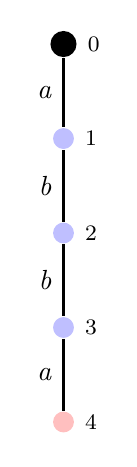
\begin{tikzpicture}[thick, level 1/.style={sibling distance=40mm}, level 2/.style={sibling distance=20mm}, level 3/.style={sibling distance=16mm}, level 4/.style={sibling distance=8mm},level 5/.style={sibling distance=4mm} xscale=-1, scale=.8]

\node[circle, fill=black] [label=right:{\footnotesize $0$}] {}
    child {node[circle,minimum width = .2cm,fill=blue!25, scale=.8] [label=right:{\footnotesize $1$}] {}
        child {node[circle,minimum width = .2cm,fill=blue!25, scale=.8] [label=right:{\footnotesize $2$}] {}
            child {node[circle,minimum width = .2cm,fill=blue!25, scale=.8] [label=right:{\footnotesize $3$}] {}
                child {node[circle,minimum width = .2cm,fill=red!25, scale=.8] [label=right:{\footnotesize $4$}] {}
                edge from parent node[left] {\textit{a}}
                }
                edge from parent node[left] {\textit{b}}
            }
            edge from parent node[left] {\textit{b}}
        }
        edge from parent node[left] {\textit{a}}
    };
\end{tikzpicture}
\end{center}

Получили такой <<бамбук>>. Теперь в дереве мы имеем перфиксы $\varnothing$ (корень), $a$, $a$ --- $b$, $a$ --- $b$ --- $b$ и $a$ --- $b$ --- $b$ --- $a$. У следующего слова с текущим деревом есть общий префикс $a$ --- $b$, поэтому мы будем не создавать новую ветку от корня, а идти по старой до конца общего префикса. Тогда наш бор приобретает следующий вид:

\begin{center}
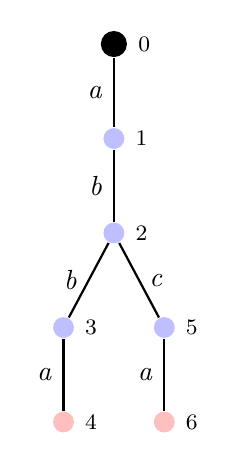
\begin{tikzpicture}[thick, level 1/.style={sibling distance=40mm}, level 2/.style={sibling distance=20mm}, level 3/.style={sibling distance=16mm}, level 4/.style={sibling distance=8mm},level 5/.style={sibling distance=4mm} xscale=-1, scale=.8]

\node[circle, fill=black] [label=right:{\footnotesize $0$}] {}
    child {node[circle,minimum width = .2cm,fill=blue!25, scale=.8] [label=right:{\footnotesize $1$}] {}
        child {node[circle,minimum width = .2cm,fill=blue!25, scale=.8] [label=right:{\footnotesize $2$}] {}
            child {node[circle,minimum width = .2cm,fill=blue!25, scale=.8] [label=right:{\footnotesize $3$}] {}
                child {node[circle,minimum width = .2cm,fill=red!25, scale=.8] [label=right:{\footnotesize $4$}] {}
            edge from parent node[left] {\textit{a}}
                }
            edge from parent node[left] {\textit{b}}
            }
            child {node[circle,minimum width = .2cm,fill=blue!25, scale=.8] [label=right:{\footnotesize $5$}] {}
                child {node[circle,minimum width = .2cm,fill=red!25, scale=.8] [label=right:{\footnotesize $6$}] {}
            edge from parent node[left] {\textit{a}}
                }
            edge from parent node[right] {\textit{c}}
            }
        edge from parent node[left] {\textit{b}}
        }
    edge from parent node[left] {\textit{a}}
    };
\end{tikzpicture}
\end{center}

Следующее слово не имеет общих префиксов с уже добавленными (на самом деле имеет, просто пустой), поэтому его подвешиваем к корню:

\begin{center}
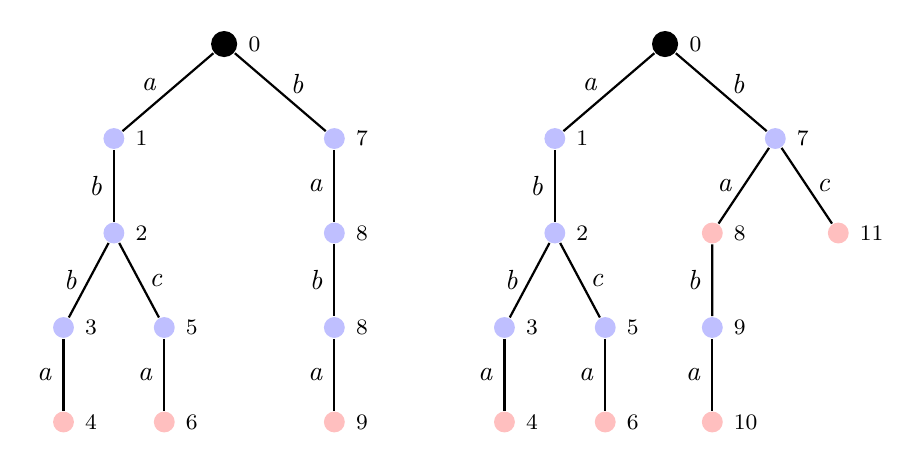
\begin{tikzpicture}[thick, level 1/.style={sibling distance=35mm}, level 2/.style={sibling distance=20mm}, level 3/.style={sibling distance=16mm}, level 4/.style={sibling distance=8mm},level 5/.style={sibling distance=4mm} xscale=-1, scale=.8]

\node[circle, fill=black] [label=right:{\footnotesize $0$}] {}
    child {node[circle,minimum width = .2cm,fill=blue!25, scale=.8] [label=right:{\footnotesize $1$}] {}
        child {node[circle,minimum width = .2cm,fill=blue!25, scale=.8] [label=right:{\footnotesize $2$}] {}
            child {node[circle,minimum width = .2cm,fill=blue!25, scale=.8] [label=right:{\footnotesize $3$}] {}
                child {node[circle,minimum width = .2cm,fill=red!25, scale=.8] [label=right:{\footnotesize $4$}] {}
            edge from parent node[left] {\textit{a}}
                }
            edge from parent node[left] {\textit{b}}
            }
            child {node[circle,minimum width = .2cm,fill=blue!25, scale=.8] [label=right:{\footnotesize $5$}] {}
                child {node[circle,minimum width = .2cm,fill=red!25, scale=.8] [label=right:{\footnotesize $6$}] {}
            edge from parent node[left] {\textit{a}}
                }
            edge from parent node[right] {\textit{c}}
            }
        edge from parent node[left] {\textit{b}}
        }
    edge from parent node[left, yshift=.1cm] {\textit{a}}
    }
    child {node[circle,minimum width = .2cm,fill=blue!25, scale=.8] [label=right:{\footnotesize $7$}] {}
        child {node[circle,minimum width = .2cm,fill=blue!25, scale=.8] [label=right:{\footnotesize $8$}] {}
            child {node[circle,minimum width = .2cm,fill=blue!25, scale=.8] [label=right:{\footnotesize $8$}] {}
                child {node[circle,minimum width = .2cm,fill=red!25, scale=.8] [label=right:{\footnotesize $9$}] {}
                edge from parent node[left] {\textit{a}}
                }
                edge from parent node[left] {\textit{b}}
            }
            edge from parent node[left] {\textit{a}}
        }
        edge from parent node[right, yshift=.1cm] {\textit{b}}
    };

\scope[xshift=7cm]
\node[circle, fill=black] [label=right:{\footnotesize $0$}] {}
    child {node[circle,minimum width = .2cm,fill=blue!25, scale=.8] [label=right:{\footnotesize $1$}] {}
        child {node[circle,minimum width = .2cm,fill=blue!25, scale=.8] [label=right:{\footnotesize $2$}] {}
            child {node[circle,minimum width = .2cm,fill=blue!25, scale=.8] [label=right:{\footnotesize $3$}] {}
                child {node[circle,minimum width = .2cm,fill=red!25, scale=.8] [label=right:{\footnotesize $4$}] {}
            edge from parent node[left] {\textit{a}}
                }
            edge from parent node[left] {\textit{b}}
            }
            child {node[circle,minimum width = .2cm,fill=blue!25, scale=.8] [label=right:{\footnotesize $5$}] {}
                child {node[circle,minimum width = .2cm,fill=red!25, scale=.8] [label=right:{\footnotesize $6$}] {}
            edge from parent node[left] {\textit{a}}
                }
            edge from parent node[right] {\textit{c}}
            }
        edge from parent node[left] {\textit{b}}
        }
    edge from parent node[left, yshift=.1cm] {\textit{a}}
    }
    child {node[circle,minimum width = .2cm,fill=blue!25, scale=.8] [label=right:{\footnotesize $7$}] {}
        child {node[circle,minimum width = .2cm,fill=red!25, scale=.8] [label=right:{\footnotesize $8$}] {}
            child {node[circle,minimum width = .2cm,fill=blue!25, scale=.8] [label=right:{\footnotesize $9$}] {}
                child {node[circle,minimum width = .2cm,fill=red!25, scale=.8] [label=right:{\footnotesize $10$}] {}
            edge from parent node[left] {\textit{a}}
                }
            edge from parent node[left] {\textit{b}}
            }
        edge from parent node[left] {\textit{a}}
        }
        child {node[circle,minimum width = .2cm,fill=red!25, scale=.8] [label=right:{\footnotesize $11$}] {}
        edge from parent node[right] {\textit{c}}
        }
    edge from parent node[right, yshift=.1cm] {\textit{b}}
    };
\endscope
\end{tikzpicture}
\end{center}

Аналогично добавляем в бор остальные слова. Заметим, что терминальные вершины (помечены красным на иллюстрациях) не обязательно должны быть листьями деревьев. Теперь научимся по данному префиксу находить количество слов с таким префиксом. Будем определять префикс по его конечной букве (конечной вершине бора). Понятно, что для листовых вершин (которые обязательно являются терминальными) ответ --- $1$. А для каждой следующей действует следующее правило: искомое число равно сумме входящих значений входящих в неё вершин. Также нужно прибавить $1$, если данная вершина является терминальной.

Следует также помнить, что бор можно строить не только на строках, а на двоичных представлениях чисел. В такой структуре вставка и поиск работают за $O(|n_2|)$, где $n_2$ --- двоичная строка, представляющая число $n$.

\subsubsection{Реализация}

\begin{minted}[linenos, mathescape]{cpp}
// нам нужны ссылки на все буквы
vector<vector<int>> link(1, vector<int>(26, -1));
// для каждой вершины отмечаем, является ли она терминальной
vector<int> marks(1, 0);

// функция для вставки слова в бор
// передаём не саму строку, а ссылку на неё, это работает за 
// $O(1)$, а не $O(|s|)$
void insert(string& s)
{
    int v = 0;
    for (int i = 0; i < int(s.size()); ++i)
    {
        int to = s[i] - 'a';
        if (link[v][to] == -1)
        {
            // Создаём новую вершину
            link.emplace_back(26, -1);
            link[v][to] = int(marks.size()) - 1;
            marks.push_back(0);
        }
        v = link[v][to]; // переходим к новой вершине
    }
    marks[v]++;
}

bool find(string& s)
{
    int v = 0;
    for (int i = 0; i < int(s.size()); ++i)
    {
        int to = s[i] - 'a';
        if (link[v][to])
            return false;
    }

    return marks[v];
}
\end{minted}

\subsection{Хеши}

\begin{definition}[\textit{Прямой полиномиальный хеш}]
    $h(s) \vcentcolon = s_0 + s_1k + s_2k^2 \hm + \ldots + s_nk^n \pmod p$, где $k$ --- произвольное число, большее размера алфавита, а $p$ --- достаточно большой модуль.
\end{definition}

Его можно подсчитать за линейное время, поддерживая переменную, равную $k$ в нужной степени:

\begin{minted}[linenos, mathescape]{cpp}
long long h = 0, m = 1;

for (char c : s)
{
    int x = (int)(c - 'a' + 1);
    h = (h + m * x) % mod;
    m = (m * k) % mod;
}
\end{minted}

Используя тот факт, что хеш --- это значение многочлена, можно быстро пересчитывать хеш от результата выполнения многих строковых операций. Например, так можно посчитать хеш от конкатенации строк $a$ и $b$: $h(ab) = h(a) + k^{\abs{a}} \cdot h(b)$. Удалить префикс строки можно так: $h(b) = \frac{h(ab) - h(a)}{k^{\abs{a}}}$, суффикс --- так: $h(a) = h(ab) - k^{\abs{a}} \cdot h(b)$.

В задачах нам часто понадобится домножать $k$ в какой-то степени, поэтому имеет смысл предпосчитать все нужные степени и сохранить в массиве $p$.

Как это использовать в реальных задачах? Пусть нам надо отвечать на запросы проверки на равенство произвольных подстрок одной большой строки. Подсчитаем значение хеш-функции для каждого префикса:

\begin{minted}[linenos, mathescape]{cpp}
vector<int> h;
h[0] = 0;

for (int i = 0; i < n; ++i)
    h[i + 1] = (h[i] + p[i] * s[i]) % mod;
\end{minted}

Теперь с помощью этих префиксных хешей мы можем определить функцию, которая будет считать хеш на любом подотрезке: $h([s_l\ldots, s_r]) \hm = \frac{h_r - h_l}{k^l}$. Деление по модулю возможно делать только при взаимно простых $k$ и модуля. В любом случае, можно этого избежать. Для нашей задачи неважно получать именно полиномиальный хеш --- достаточно, чтобы наша функция возвращала одинаковый многочлен от одинаковых подстрок. Вместо приведения к нулевой степени приведём многочлен к какой-нибудь достаточно большой, например, к $n$-й: $h([s_l\ldots s_r]) = k^{n - l}(h_r - h_l)$. Так проще --- теперь нужно домножать, а не делить:

\begin{minted}[linenos, mathescape]{cpp}
int hash_substring(int l, int r)
{
    return (h[r + 1] - h[l]) * p[n - l] % mod;
}
\end{minted}

Теперь мы можем просто вызывать эту функцию от двух отрезков и сравнивать числовое значение, отвечая на запрос за $O(1)$.


\section{Парадигмы программирования (бонус)}

\subsection{Процедурное программирование}
Обычно код, который пишется для олимпиадного программирования - процедурный.
Это значит, что программа состоит из последовательности инструкций (функций), изменяющих состояние
(изменяет и использует переменные в глобальной области, а не только на аргументы)\\
\textbf{Отличительные черты:}

- \textbf{Императивный стиль}: программа — это последовательность команд.

- \textbf{Функции} как основные блоки кода (не привязаны к объектам).

- \textbf{Быстр} в написании, но неудобен в чтении сторонним разработчиком

- \textbf{Сложен} в поддержке крупных проектов

- Есть переменные в \textbf{глобальной области}

\subsection{Объектно-ориентированное программирование (ООП)}
Думаю, любой начинающий программист задумывался: ``Можно ли создать свой тип данных?'', и ответ - да.
Главная черта ООП - создание своих типов данных

Решение большинства задач через ООП зачастую требует большого времени, чем через процедурное программирование,
зато другой человек сможет понять и использовать его в разы быстрее, поэтому он идеален для создания библиотек.
Например, std::vector, std::string, std::map, std::set и многие другие написаны через классы.
Вообще всё, что не является примитивом (то есть числом, ссылкой или указателем)
В олимпиадном программировании самый подходящий пример для ООП пример - СНМ.

В c++ есть две синтаксические конструкции для создания типов данных: структуры (пришли ещё из языка си) и классы.

\vspace{0px}
\subsubsection{Начнём со структур}

Базовый синтаксис:

\begin{minted}[linenos, mathescape]{cpp}
struct Struct { // где struct - ключевое слово, Struct - имя структуры

}; // почему-то в конце нужни ';'
\end{minted}

Внутри структуры можно хранить данные (они называются не переменными, а полями):

\begin{minted}[linenos, mathescape]{cpp}
struct Struct {
    int n = 0; // можно ставить значение по умолчанию
    std::vector<int> array; // можно использовать любые типы данных
};

int main() {
    Struct test; // создание объекта структуры
    test.n = 54; // присвоение
    cout << test.n; // вывод
    test.array.resize(10); // можно вызывать методы у полей
}
\end{minted}

У структуры могут быть методы (функции), например push\_back у std::vector

\begin{minted}[linenos, mathescape]{cpp}
struct Struct {
    int n = 0;
    std::vector<int> array;

    void setSize(int n_) {
        n = n_;
        array.resize(n_);
    }
};

int main() {
    Struct test;
    test.setSize(10);
}
\end{minted}

Когда мы создаём std::vector, мы часто указываем длину (std::vector array(10)), когда мы так делаем, мы вызываем
конструктор - особый метод, который вызывается при создании объекта структуры/класса.
У него нет возвращаемого типа (даже не void), а называется он так же как и структура/класс

\begin{minted}[linenos, mathescape]{cpp}
struct Struct {
    int n = 0;
    std::vector<int> array;

    Struct(int n_) {
        n = n_;
        array.resize(n_);
    }
};

int main() {
    Struct test(10);
    Struct test2; // будет ошибка
}
\end{minted}

Конструкторов может быть много:

\begin{minted}[linenos, mathescape]{cpp}
struct Struct {
    int n = 0;
    std::vector<int> array;

    Struct() {}

    Struct(int n_) {
        n = n_;
        array.resize(n_);
    }

    Struct(const std::vector<int>& array_) {
        n = array_.size();
        array = array_;
    }
};

int main() {
    Struct test0;
    Struct test1(10);
    std::vector<int> array(10);
    Struct test2(array);
}
\end{minted}

\subsubsection{Инкапсуляция — сокрытие данных}

В структурах присутствуют модификаторы доступа: public, private, protected.
По-умолчанию все поля и методы - public, но давайте представим, что мы бы могли менять переменную, отвечающую за размер,
в таком случае мы бы могли назначить, например, отрицательное значение, и этим всё сломать.
Давайте, для примера, в нашей структуре сделаем так, чтобы нельзя было менять n вне зависимости от array.
Чтобы изменить размер, придётся вызывать setSize.

\begin{minted}[linenos, mathescape]{cpp}
struct Struct {
private:
    int n_ = 0; /* private поля и методы принято маркировать _ в конце
        имени, но это не обязательно */
    std::vector<int> array_;

public:
    int getSize() {
        return n;
    }

    void setSize(int n0) {
        n_ = n0;
        array_.resize(n0);
    }
};

int main() {
    Struct test;
    test.setSize(10);
    cout << test.getSize();
    cout << test.n_; // будет ошибка
    test.n_ = 54; // будет ошибка
}
\end{minted}

Есть ещё protected, но он нужен при наследовании, а на олимпиадах в его использовании смысла нет.

\subsubsection{Классы}

В c++ классы и структуры различаются только модификаторами доступа по умолчанию в структурах - public, а в классах - private

\begin{minted}[linenos, mathescape]{cpp}
class Struct {
private: // можно не писать
    int n = 0;
    std::vector<int> array;

public:
    int getSize() {
        return n;
    }

    void setSize(int n_) {
        n = n_;
        array.resize(n_);
    }
};
\end{minted}

\subsubsection{Константные методы}

Пусть дан код:

\begin{minted}[linenos, mathescape]{cpp}
class Struct {
    int n = 0;
    std::vector<int> array;

public:
    int getSize() {
        return n;
    }

    void setSize(int n_) {
        n = n_;
        array.resize(n_);
    }
};

void func(const Struct& struct) {
    struct.getSize() // даст ошибку
}
\end{minted}

Этот код не скомпилируется, так как метод getSize не константен.
\textit{Константные методы} - методы, которые не меняют поля класса (могут вызывать только константные методы).
Это можно исправить так:

\begin{minted}[linenos, mathescape]{cpp}
    int getSize() const {
        return n;
    }
\end{minted}

Также константные методы лучше помечать [[nodiscard]].
Это заставит компилятор выдать warning, если возвращаемое значение не было использовано.

\begin{minted}[linenos, mathescape]{cpp}
    [[nodiscard]] int getSize() const {
        return n;
    }
\end{minted}

\newpage
\thispagestyle{empty}

%\noindent
%\topskip0pt
%\vspace*{\fill}
%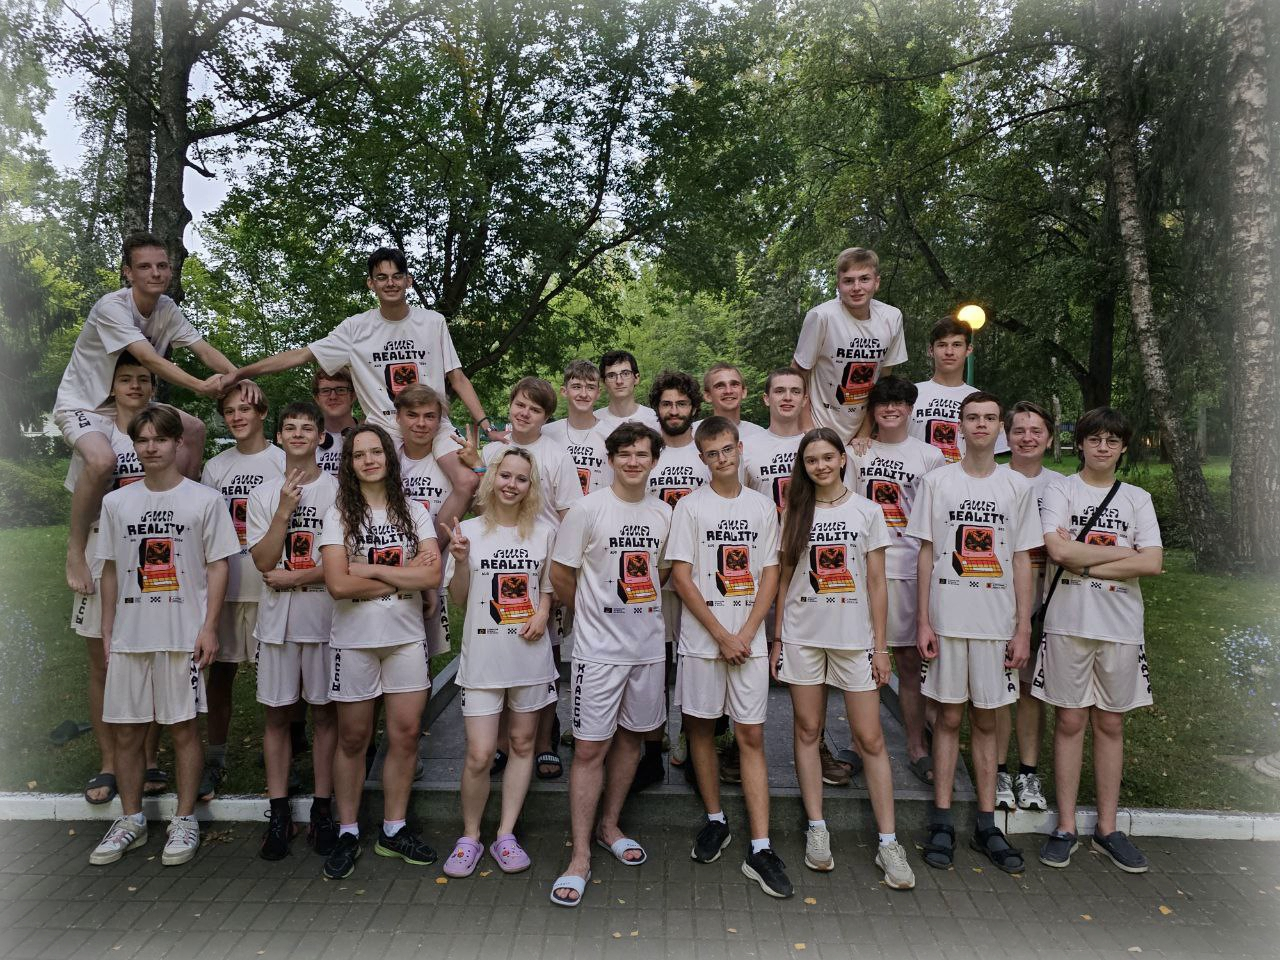
\includegraphics[width=\textwidth]{./img/final_photo.jpg}

\end{document}

% TODO динамика по цифрам и профилю
